\documentclass[11pt]{report}
\usepackage[a4paper,margin=10mm,footskip=5mm]{geometry}
\usepackage{color}
\usepackage{titlesec}
\usepackage{setspace}
\usepackage{enumitem}
\usepackage[utf8]{inputenc}
\usepackage{graphicx}
\usepackage{wrapfig}
\graphicspath{ {./img/} }

\renewcommand{\rmdefault}{lmtt}
\renewcommand{\sfdefault}{lmtt}
\renewcommand{\ttdefault}{lmtt}

\renewcommand*\footnoterule{}

% Itemize and enumerate settings
\setlist{noitemsep}
\setlist{nosep}
\setitemize[0]{leftmargin=*}

% These values are offset-values from the default margins.
\setlength{\hoffset}{-1in}
\setlength{\oddsidemargin}{25mm}
\setlength{\evensidemargin}{25mm}
\setlength{\textwidth}{160mm}

\addtolength{\topmargin}{4mm}
\addtolength{\textheight}{-12mm}

\setlength{\parindent}{0mm}
\setlength{\parskip}{0.5em}
\renewcommand{\baselinestretch}{1.15}

\renewcommand{\labelitemi}{$-$}
 
\titleformat
{\chapter} % command
[hang] % shape
{\huge} % format
{} % label
{0ex} % sep
{\hspace{-0.4pt}\thechapter\hspace{0.6em}} % before-code
[] % after-code
 
\titleformat
{\section} % command
[hang] % shape
{\LARGE} % format
{} % label
{0ex} % sep
{\hspace{-0.4pt}\thesection\hspace{0.6em}} % before-code
[] % after-code

\titleformat{\subsection}[hang]{\Large}{}{0em}
{\hspace{-0.4pt}\thesubsection\hspace{0.6em}}[]

\titleformat{\subsubsection}[hang]{\large}{}{0em}
{\hspace{-0.4pt}\thesubsubsection\hspace{0.6em}}[]

\titleformat{\paragraph}[hang]{\bfseries\normalsize}{}{0em}{}[]

\titlespacing{\chapter}{0em}{0.5em}{0em}{}
\titlespacing{\section}{0em}{0.5em}{0em}{}
\titlespacing{\subsection}{0em}{0.5em}{0em}{}
\titlespacing{\subsubsection}{0em}{0.5em}{0em}{}
\titlespacing{\paragraph}{0em}{0.5em}{0em}{}


\begin{document}


\vspace*{3cm}
\begin{center}
\uppercase{
\fontsize{3.4cm}{3.4cm}\selectfont
Pr0mans\\
\fontsize{1.5cm}{2cm}\selectfont Tutorial to the\\
\fontsize{2.5cm}{2.5cm}\selectfont Apocalypse}\\
\normalsize \vspace{5cm} \today
\end{center}

\tableofcontents

\raggedright
\chapter{Introduction}
 
Since the C:DDA-Discord grows each day, the community constantly raises beginners' questions regarding the start of a new game so I've decided to put out a (hopefully) comprehensive manual to Cataclysm: Dark Days Ahead, that will cover most of the things encountered in the game. This Text will, over the course of the creation, cover all the basic things: Character creation, The base game and it's most important controls, guides to the various stages of the game (played by me on basic settings) as well as several parts of the games' explanation in-depth.
The reasoning for me writing a guide, or at this point, tutorial rather to begin with is simple - all the information found for this game is incredibly dated and therefore I wish to put up a comprehensive knowledge-book for newcomers to be pointed to if they wish to learn more about the game but also for veterans to check out again if they lack some information or just want to refresh their memory after being absent for ages.
So before we start, some info about me: I'm Pr0man, a somewhat dated veteran of the game who played this back when it was just called "Cataclysm" (C:DDA is technically a fork of the original). I'm more often than not streaming the game on twitch and I usually play with some pretty hard world settings, so be aware that this guide may or may not be biased towards a more careful playstyle. I am certain that I have a good understanding of the general mechanics of the game, as well as some in-depth knowledge of some other intricacies the game can throw at you without warning.
HOWEVER - I am by no means all-knowing and therefore you should be careful that some topics may not contain correct or proper information to boot. I tried collecting knowledge from many different sources in order to compile them into this wordy document, but remember to take in all of that with a grain of salt. Feel free to correct me, to ask me certain things or whatever you feel could be done to improve this piece of work I try to call a "tutorial".

While the game has changed drastically over the course of its development, many questions have not. And after answering many questions over and over again, I decided it is time to put my wasted energy into writing this. And without further ado, let's get to the meat of things.

 
\chapter{Overview of Controls}
 
Since Cataclysm: Dark Days Ahead is an ASCII Game (a complex one at that), the control scheme is different from the modern day type of games. You will be required to utilize all of your keyboards' buttons to get every possible action done. Another factor is the capitalization of letters. so [e] is another Button altogether than [E].
 
Movement is done either by using the keyboard's numeric keyPad, with each of the buttons representing one of the 8 directions and [5] being the vvvvvvvvvvvvvvvvvvvv option. There is also the option of using a different control layout using the right side of the keyboard, yet this is probably more difficult to use.

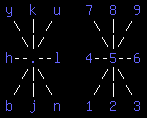
\includegraphics{01}

Buttons of interest:

[@] - character overview \newline
[i] - inventory screen \newline
[E] - consume an item from inventory or close by \newline
[a] - use an item from inventory or close by \newline
[A] - activate currently held item \newline
[d] - drop something \newline
[D] + directional input - drop something onto that location\newline
[e] + directional input - examine something that lies in the direction you gave input to. This allows for pickup from a location, like taking something from a freezer or oven and can open contextual menus (e.g. Curtains)\newline
[\%] - contextual menu - this is a comprehensive list of actions you can perform with the tools and items at hand.\newline
[x], [;] - Look around, this lets you freely move the camera around your field of view.\newline
[TAB] - auto-attack nearby enemies (including at range if you wield a weapon with reach)\newline
[X] + directional input - peek around that location, perfect for peeking around corners, as it will allow to see what is around without those actually notice you.\newline
[o] - open a door\newline
[c] - close a door\newline
[s] + directional input - smash something in that location\newline
[g], [,] - pick up items\newline
[G] - grab Item/Furniture - allows you to pull things along, like small vehicles, bookcases and the likes.\newline
[B] - butcher something you are standing on, also allows for disassembly if you meet the requirements.\newline
[V] - list everything around the player that is in sight. this can be toggled to monster view or item view using [TAB] and [s]-orted into either category or range to player\newline
[W] - wear item that is nearby or in your inventory\newline
[T] - take off a piece of clothing\newline
[w] - wield item nearby or in your inventory\newline
[R] - read something\newline
[r] - reload items that require ammunition\newline
[U] - unload item\newline
[t] - throw something\newline
[f] - fire held item\newline
[p] - open the Bionics' overview\newline
[\^] - control vehicle, if used on a tile that has no controls, allows for input to open the vehicles' control menu\newline
["] - toggle sprint/walk\newline
[\$] - go to sleep\newline
[\&] - crafting menu\newline
[*] - construction menu\newline
[\textbackslash] - haul items on the ground\newline
[/] - advanced inventory screen\newline
[[] - Open mutations screen - allows to activate/toggle eligible mutations
 
Remember - keys can be rebound and this is only a small selection for those that want to get a general idea of what does what. Consult the keybindings menu for a full overview of all the keys. 

\chapter{World}

When selecting new game, you are asked to basically create a new world from scratch, though this option can also be done from the [W]orld option in the main menu. it'll bring you to the exact same screen. There you will be asked to include or exclude mods for the extra experience.
On the mod list screen you can move around the inner screen in which you can select mods using the arrow keys and add/remove them using Enter. cycle through the mod tabs [default], [Blacklist] and [Balance] using [>] and [<] respectively, and move through the top rosters [World Mods], [World Options] and [Finalize World] using [TAB] and [Shift] + [Tab].

So with this in mind, we could include some mods. For the sake of this Tutorial, we shall only include the base game and the mods that are standard active - Meaning the C:DDA Core, Filthy Clothing, Disable NPC Needs and Simplified Nutrition.

How do we set up our world though? What do the different numbers and scales do exactly and what would be considered to be an easy game or hard game?


\section{The Creation}

World end Handling - Keep/Reset/Delete -> Basically allows you to tell the game what happens to the world once you die. I personally prefer to play using the Reset settings, as starting in a location that has been looted by a previous character can be utterly frustrating.

Size of Cities - [0 to 16] -> this setting sets the scaling factors to city generation. Remember that even with very small or very big numbers, size of cities can vary drastically. The base value of 8 (increased from 4 as of version 8400)  generates town of sizes ranging from 10 houses up to big cities with over 100 buildings. Generally ranging somewhere from 40-70 based on observation. I'd go with a 10.

City Spacing - [0 to 8] -> This setting in turn is an indicator for how close cities are going to be generated to each other. Smaller numbers mean cities are closer together, while a spacing of 6+ makes for day long travels, even with a vehicle. Go with 4 for the best results for the first world.

Spawn Rate Scaling Factor [0.00 to 50.00] -> Sets the amount of monster spawning, a value of 0 would deactivate spawning all together, while a value of 2 would effectively double the amount of monsters. Small changes can already have a huge impact on monster density inside a town, especially when paired with Wanders Spawns: On.

Carrion Spawn Rate scaling factor [0\% to 1000\%] -> Sets the value at how often (and therefore how quick) critters spawn out of rotten edibles, a value of 0\% disables this mechanic all together.

Item Spawn scaling factor [0.01 to 10.00] -> Sets the amount of items found in certain locations. This does not impact monster drop tables and is only meant to influence how many items are spawned in any given spot.
NPC Spawn Rate scaling factor [0 to 100.00] -> sets the density and thereby the chance of an NPC spawning in on the edge of your reality bubble (more on that in chapter 5.3.10). This does only influence randomly spawned in NPCs, not static NPCs. If you wish to encounter NPCs on a regular basis, set this value to 1 - 1.5, for the odd encounter maybe 0.5

Monster Evolution scaling factor [0.00 to 100] -> sets the time required for a monster to spawn 1 evolution category higher than it normally would have. 0 disables evolution of monsters, a higher number means more days need to pass for evolution to occur. If you have trouble with high-power zombies, increase this value, other than that, decrease it - I'd suggest going with 15-30

Monster Speed/Resilience [1\% to 1000\%] -> This multiplies both the internal speed and HP that each monster is spawned with. A lower number means the monsters are gonna be slower and take less hits to kill, while a higher number will make them tougher and faster respectively.

Default region type [default] -> This feature is not yet implemented, but planned to be able to switch to different regions to play in, like deserts.

Initial Time [0 to 23] -> this sets the time of the current world upon spawn, 0 meaning midnight, 12 midday etc.

Initial Season [Spring, Summer, Autumn, Winter] -> Sets the season the world is currently in when spawning a new character. Note that the season will have severe impacts on the availability of food as well as the temperature outside. Summer is easy to start out in, as clothing isn't as important and food is readily available. I'd still suggest using spring out of nostalgia reasons, they got a bit harsher.

Season Length [14-91] -> Amount of days required till a season switches from one to the next. I'd say go with 30-45

Construction Scaling [0 to 1000] -> Scales the speed in percent that each construction would take. 50 doubles it, 200 halves the speed. 0 scales the time proportionally to your season length, which can cause you to construct very slowly.
Eternal Season [false/true] -> When this setting is enabled, the seasons will not cycle and you will be trapped in the starting season selected.

Wander Spawns [false/true] -> This setting allows for a sound based repositioning of zombies from one location to another by taking monsters from a pool of nearby structures and teleporting them relatively close to the sound of noise, if the noise breaks a threshold. Considering that worlds are technically endless, this is just a fancy description to enable dynamic spawn. Your first couple of games should potentially be played without this feature, unless you are daring.

Classic Zombies [false/true] -> this setting will enable/disable the spawning of more exotic zombies and wildlife and keep the game to a certain degree of realism, as realistic as a zombie apocalypse can be. Overmap specials that are dedicated to those monsters will also be disabled by this setting.

Surrounded Start [false/true] -> when enabled, upon spawn you will have several zombies close by. Beware that this will also spawn in zombies from mods, if you have them (especially deadly with Cata++ and PK's mod)

Static/Random NPCs [false/true] -> When enabled, will allow for structures that contain them to be spawned in with static NPCs, while Random NPCs will be randomly spawned at the edge of your reality bubble during your gameplay.

Mutation by Radiation [false/true] -> when disabled, this will block radiation from causing you to randomly mutate, given certain thresholds.

Experimental Z-Levels [false/true] -> when enabled, will cause the game to run slower, depending on surrounding entities, but allows for enemies and allies to traverse between Z levels in a realistic manner, as sound, scent and vision will travel between those Z levels where appropriate.

Character Point Pools [Any, Multipool, No freeform] -> sets the selectable character point pools when starting a new character in the appropriate world. Any allows for any selection, Multipool restricts you to using Multipool only, No Freeform disables that option.

With all of those settings in mind, what would a newcomer to the game chose to have a relatively balanced game?

Not only is this question difficult to answer, as every person has different preferences, but every person also enjoys a different challenge. Some just want to worry about basic survival, some want to struggle in combat.

I'd suggest you don't tweak any of the Zombie modifying values (Speed/resilience/Classic/Surrounded) until you deem it necessary - while this makes for a more challenging game overall in terms of enemy variety, you will miss a lot of the games' content. Wander Spawns should either be set to on or off according to taste - I personally enjoy the extra challenge of having to deal with noise and hordes roaming around the map, though it makes clearing a city significantly more difficult. As stated earlier, I highly advise against using wander spawns if you are a newcomer to this game, as the amount of zombies that will be in towns can quite easily overwhelm you. Same goes for experimental Z-Levels, having to be careful with sound and light, even across Z-Levels makes for a great challenge on managing your survival as you can't just hide out in a basement, go to sleep in order to heal up damage you have taken, go back out again and attack. Hordes that are chasing you will actively chase after you over multiple levels, which means you can potentially trap yourself by thinking a basement or upstairs on a building is safe.

Settings you can safely modify would be: Zombie Spawn Rate (set it to 1.00 or lower if deemed necessary), carrion spawn rate (either disable it by setting it to 0 or leave it at 100\%) Item spawn rate I'd actually suggest bumping up to 1.25 or 1.5, while this makes the early game substantially easier to deal with, limitless frustration makes the game experience less enjoyable to begin with. Reducing this setting at a certain skill level, to not get handed everything right from the get-go makes for great runs later down the line. Static NPCs should be enabled, as it will populate some of the buildings you come across, otherwise those will be completely empty to begin with, namely the Refugee Center.
I'd suggest against playing with random NPCs, as they are currently horrendously unbalanced and can spawn with extremely high skills and if that NPC is considering you to be a threat, he might decide to put you out of your misery. If you want an experience like DayZ, except fun, go for it and bump up the NPC spawn rate to 0.25 first, increasing it as you see fit, but don't come crying that I didn't warn you.
Season length should be around 30, maybe even lower so you can see the effects of the appropriate seasons to the surrounding world. As this changes ambient temperature as well as what you can forage in the wilds, quicker times means more dynamics. While you will enter difficult seasons earlier, they will also pass earlier, requiring a lower stockpile.

Nevertheless I feel that it should be addressed that all of these settings are my own personal preferences - beware that some of these settings can easily make your game harder or easier, often to a dramatic degree.

\section{Mods}

(Information provided by Shard from the C:DDA Discord)
Mods for CDDA are structured as a folder that goes in cdda/data/mods, with the first level of the folder including a file called modinfo.json - besides this they can contain other files either directly or within subfolders.  Typically mods are downloaded as a zipped file either containing loose files or a folder for the mod with the files contained inside, while sometimes (typically from github) you might get something that ends up being similar to 'mymod-master/mymod/modinfo.json' at which point you need to move the mymod folder to data/mods instead of the mymod-master, as otherwise your modinfo.json would not be one layer of folders below mods/ as it should be.

Some mods require LUA support in your game.  If you downloaded an already compiled version, this is the default, and you do not have to do anything.  If you compile on your own, you need to follow the instructions for adding LUA support, as it is not default.

Most mods can be safely added or removed midgame by editing saves/worldname/mods.json and adding/removing the mod's identifier from the modinfo.json for that mod (vehicle additions pack is 'blazemod' for example, so it isn't always what you would guess)  Mods that cannot be safely added to saves: Anything that adds NPC factions.  Mods that can be tricky to remove: Anything that adds terrain (like grass/dirt/concrete) because that leaves literal holes in the world, and anything that adds new building types (spam of errors when near them, so you have to explore a new area after removing them and prune your save file to remove the old space)

For the mods that are unsafe to add due to factions being added, you can create a new game with those mods and copy the specific missing faction data from master.gsav in the new game into your old game, and then add the mod to the old save.  Be sure to back up your save file before doing so, as being unsuccessful at trying to add a mod that adds factions can corrupt your save.

\section{Suggested Mods for a Game}

(To find downloads for the newest versions, check the C:DDA Discord)
Many people have different wishes in what they'd like to have from a mod, some just like extra content, some like challenges, some just wanna breeze through the game. Nevertheless, here's a small list of Mods that I feel are well worth the addition to your game:

Arcana - provides a bunch magical related areas and items, for those that wanna see more of an occult version of cataclysm.

Artyoms' Gun Emporium - Reloaded, Icecoons Arsenal, DeadLeaves' Fictional Guns, Craftable Guns, Extended Realistic Guns - All things guns, any of the gunmods you find on the list should be added for the extra variety, even though this'll spawn so many ammo types and weapons you'll sometimes struggle to find the appropriate ammo. If the base game is lacking a firearm, you might come across something similar just by playing with these mods installed.

Cars to Wrecks - (recommended for intermediate players) -
(careful, this mod is known to behave in wonky ways) - this will cause many of the vehicles you come across in towns, roads, buildings etc. to be wrecked beyond usage, so you have to scavenge for parts that you wish to use, building vehicles from scratch, unless you get lucky. This will make you value your deathmobile even more, as spare parts are gonna be a rarity unless you make them yourself.

Cata++ - Adding not just a whole lot of enemies, but also hefty items, it's worthwhile to pick up just to engage some enemies that'll gladly kill you on long range, while packing some heavy rewards, like armor and mid to late game weapons.

PK's Rebalancing - The big daddy of mods - adding not only a whole lot of new enemies, new items and new effects but also increasing the difficulty by a notch or twelve? Weather effects are harsher, poison more crippling and enemies radiate you when struck in combat, slowly at least. For those that wish for more of a challenge while playing, this is the mod for you. To compensate for it though, you get some nice quality of life effects, lots of extra items and many new locales to explore.

Medieval Weapons - for the knights in shabby armor among you, this is a mod that is more than welcome, as it adds more medieval weapons as well as a medieval swordsmanship style.

Folding Parts pack, Tanks and other Vehicles, Vehicle addition pack, boats - All things road-warrior style. These mods have many more vehicles to spawn on the overworld, and more vehicles means more variety and more fun when mowing down Z's on the road. The folding vehicle addition is in itself great, allowing you to craft foldable parts and therefore foldable cars, while tanks' well, they are tanks!

Location adding Mods - Beta National Guard Camp, Fuji's more Buildings, More Buildings, More City Locations, More Locations, Oa's additional Buildings Mod, Tall Buildings and more - To spice up your variety in city exploration, I highly recommend these mods, as otherwise your cities are gonna be a bit bleak in terms of buildings, for the most part. While the base game has certainly added more buildings to cities, having even more of them is definitely also very handy.

\chapter{Character Creation}

Once you are happy with your worlds' settings, you now can select one of different game modes to start out with. This guide will focus on the [Custom Character] selection. Once selected and the content mods are all loaded into the system, not throwing any exceptions, you are brought to the character creation screen, separated into many different categories. First you are asked to select your point pool system: Multiple Pools, Single Pool or Freeform. Multiple Pools force you to use points in their respective pools or followup pools (except for skills). So you can't just pick a bunch of negative traits and rack up the attributes. Single Pool removes these limitations and you a free to use the points at your disposal to how you see it fit. Freeform is basically a cheat mode, you can use however many points you wish. For this Tutorial, we are going with Multiple Pools.


\section{Scenarios}

Once you have made your decision, you can choose a specific scenario that you are playing. These limit you in the terms of where you spawn, as what profession you can spawn, as well as imposing certain possibilities in the trait selection and potentially coming with extra merits that need to be resolved.
I highly suggest for a newcomer to use the Evacuee scenario and staying as far away as possible from any of the 'Challenge' scenarios. Those are meant for brutally difficult runs that are each challenging in their own rights and are no fun if you have next to no clue what you are doing. For the sake of this Tutorial, we will start as an Evacuee, but some other interesting starting Scenarios also include Wilderness, Sheltered (this is a winter spawn, regardless of season settings) or Refugee.

\section{Professions}

Professions in Cataclysm: Dark Days Ahead are what you'd consider to be your background. They either cost a certain amount of points to select, or give you points in return for selecting them. From a simple no name person, up to a hunter, blacksmith or mechanic, the variety is what nails it. Every background spawns with specific items and skills that they start out their journey with. While some come with handy tools to use, great skills for their cost, some are just more challenging because of what they don't come with. Some professions spawn with not only less of a certain thing, like clothes, but also come with negatives, such as addictions to certain drugs that will severely hamper your start (I'm specifically looking at you Tweaker!). Or some might be what you consider to be powerful cyborgs that come outfitted with Bionic implants (more on that later) that can greatly change the flow of the game - in a positive as well as negative direction. Professions can however, be locked behind certain starting scenarios or be excluded from some scenarios you'd consider them to be a part of. Feel free to check out the different scenarios' starting professions. As for this guide, I assume the profession of the Survivor, the most basic of the starts available.

This leaves us with 6 Stat points, 0 Trait points and 2 Skill points for our character creation for a total of 8.

\section{Traits}

Traits are the defining, well, traits that make you who you are: A faceless, nameless git that somehow managed to survive the initial strike of the cataclysm.

Traits can affect your gameplay in a positive or negative way in many different severities. (Specific professions get a 3rd tab, profession Traits, that is unavailable to most of the characters)

While traits may seem like something you can easily gloss over, they are however extremely important when it comes to how you want to experience the game.

  Here I am going to give a quick list of traits (positive and negative) that I feel are worth picking up for several reasons:

Positive Traits:
Animal Empathy (1 point) - smaller game is less likely to run away from you, while bigger animals like dogs, wolves or moose are less likely to just charge at you and attack. And believe me, moose are well-known early game character killers. So if you have the point to spare and trouble surviving in the wilderness, consider picking this up.

Deft (1 Point) - For those melee focused characters, being able to recover from a missed swing quicker means the enemy has less time to land a hit on you. Many Weapon- and Martial Arts style come with built-in deft like abilities, so it's not something one would be picking normally, but for those that neither have access or want to avoid special weapon styles, it can be worthwhile picking up.

Disease Resistant (1 Point) - While this will only save you from the more common diseases like the flu or the common cold, being more resistant to those in particular can be great if you happen to catch one of those more often than you'd like. Limited in usefulness in general, as ailments for those illnesses are commonplace. Consider it for a wilderness run - Bee Balm tea only gets you so far after all.

Fast Healer (2 Points) - You heal damage done to your body more quickly by sleeping, you even heal very small amounts of HP while awake and limbs will heal noticeably quicker. If you feel yourself taking damage a lot, which in turn leaves you crippled in your hideout, you might want to consider grabbing this trait.

Fast Learner (3 Points) - This will make all practically earned experiences raise your skills quicker. For the amount of points it costs, the effect it has is quite low. This does exclude knowledge gained from books, has however great application when training combat focused skills, as those will rise quicker, which makes for an easier life all around by quickly gaining combat related skill levels.

Quick (3 Points) - This makes you 10\% quicker in every aspect. From walking/running, to attacking, eating and whatnot. If you require that extra bit of performance from your character and have the points to spare, this is a great pick.

Fast Reader (1 Point) - Reading books that will provide you will extra skills far quicker than getting into fist-fights all the time? Definitely a nice pick if you want to learn most of your skills from books. Remember though, for combat related skills - books only get you so far as there are no end-game books for combat skills by design. The reading time on some late game books however might just make this trait worth the single point.

Fleet-Footed (2 Points) - Feeling a bit slow in comparison to the undead? Grab this perk to be 15\% quicker while on sure footing, which relates to all things you don't require to balance upon, like boulders, railings, rubble and wreckages.

High Adrenaline (2 Points) - This perk is more of a double-edged sword than one would believe. In tense combat moments you will gain the Adrenaline Rush effect, which boosts your Str, Dex and Per, as well as numbing pain a bit, while giving you great stamina recovery. However, once it wears off it leaves you pretty vulnerable as it does reduce your stats for a time. Take at your own risk - the power boost may save your bacon.

Martial Arts Training, Melee Weapon Training, Self Defense Classes, Shaolin Adept and Venom Mob Protegee (2 to 3 points each) - What all of those traits have in common is that these traits (more like backgrounds or hobbies) will provide you with 1 of the several different Martial Arts and Weapon Arts the game has to offer. These will drastically change combat capabilities and can turn the tide in many of the different combat scenarios you may find yourself in. Anybody wanting to play a martial artist is bound to pick one of those, as a no-style unarmed combat characters' damage is significantly lower

For those that wish to become really strong early on. I'd suggest Melee Weapons Training (Eskrima) and grabbing yourself a pipe to smack enemies around with.

For a more in-depth look at the respective Martial Arts, I can only suggest you to check out this discourse post made:

https://discourse.cataclysmdda.org/t/best-unarmed-styles-for-early-game/15558/11

Night Vision (2 Points) - In my opinion an absolutely mandatory pick for any survivor out there. What this trait allows for is taking your perception and giving you 1 tile of vision for each 3 points in Perception while in complete darkness. This trait will NOT however allow you to do crafting that requires you to see or reading.

Packmule (2 points) - This perk will raise your volume capacity by 40\%. This does not include weight, which is covered by Strong Back (35\% more carry weight). This makes the most use out of all your pockets if you wish to travel in light gear and without a Backpack to keep your encumbrance low (more on encumbrance in chapter 4.2.2 - Temperature and Clothing) and is a definite pick for those that either wish to carry around some utility gear while also being clothed sparingly, or for the absolute hoarder that runs without a shopping cart.

Parkour Expert (2 Points) - Removes or lowers the movement penalty when moving through tiles that would slow you down. Railings, windows, bushes, grass, you name it. This allows you to widen the gap between you and monsters more easily. Makes for a great way of escaping, as well as a nice way to kite monsters into tiles that would slow them down, giving you more time to strike them

Pain Resistant (2 Points) - What is Pain? It's the reason you constantly die. Pain slows you down, which in relative terms, speeds up your enemies and allows them to get more hits in, it reduces your attributes quickly, sometimes drastically and it makes you miss more often in combat, which is the last thing you want while being so close to killing that last enemy. If you happen to be in pain quite often and Aspirin isn't doing it for you, consider picking this perk up to supplement it.

Psychopath (2 Points) - No guilt from killing enemies that you'd consider having scruples for. This means that killing zombie children and the likes will incur no penalty to your mood, which can quickly cripple your crafting capabilities. The perk has also the added benefit of you not caring about human life and allows you to freely kill, butcher, and eat human entities - a great extra food source.

Robust Genetic (3 points) - For those that wish to be more explorative with the inner workings of their body, this trait will make it so that mutations you receive either from outside influences (radiation, enemy attacks) or from willingly taking mutagens have a higher chance of being positive than negative. A must have for those that wish to play with mutations more.

Strong Stomach (1 Point) - This will keep your food down if you are nauseous from either drinking unclean water, which can poison you, or if you happen to get poisoned by an enemy. Works well in conjunction with the negative food traits.

Negative Traits:
Addictive Personality (+2 Points) - Addictions will hit in quicker for you, and you'll have a harder time of getting rid of them. Sounds nasty, but if you use addictive items sparingly, like the odd cigarette, or not snort meth like it's nobody's business, you are totally fine with this perk. For those interested - you'd need to take in 3 doses and be unlucky enough to get 3 addiction level increases (more on that in Chapter 6.3.1)

Animal Discord (+1 Point) - if, on the other hand, animal life is not much of a threat to you since you know what you are doing, picking up animal discord can actually be a benefit, as it will make wild game more aggressive and therefore run away less often, helping you out while hunting small and big game alike.

Far/Near-sighted (+2 Points each) - glasses are extremely common in the apocalypse, and they are also quite sturdy, so having these traits is a total non-issue for the most part. Just make sure to not take them off, as Near-sighted limits your view range dramatically, while Far-sighted prevents you from reading and using Terminals and makes hitting things in combat pretty difficult. Also guarantees you to spawn with the appropriate set of glasses when you start out.

Forgetful (+3 Points) - Forgetful causes you to lose skills due to skill rust quicker and you will forget what map tiles are what when you are far away from them for extended time. If you play with skill rust disabled, the first effect won't work and therefore gives you basically 3 free points. Even with skill rust enabled, the effect is not too terrible. (I'd suggest playing with int-capped skill rust for best effect)

Glass Jaw (+2 Points) - while having less HP on your head seems to be a pretty nasty effect, remember that helmets of many different types are pretty common inside towns, and with some tailoring you are able to craft headgear which can be pretty powerful relatively early. If you feel daring, feel free to grab this perk for some extra points.

Topographagnosia (rolls right off your tongue) (+5 Points) - said to lower your vision on the overmap, this trait doesn't prevent map exploration through events. Checking the console for the Refugee Center will still show you most of the landmarks on the way for example. If your big worry is early game, this doesn't seem like it will hurt you too much while also giving a ridiculous amount of points in return.

Trigger Happy (+1 Point) - weapons that support full auto can rarely go full auto when firing. Not only does this not apply if you aren't using firearms that don't support full auto, if you intend to not use firearms at all, or in extremely bad situations (where Full auto might save your bacon) this trait is a safe pick

Ugly and Truth teller (each +1 Point) - negative NPC Traits - If you plan to not play with NPCs, again, free points. Even when playing with NPCs, lying is too difficult without any skill in speaking and being ugly only lowers the chances of talking down NPCs or asking them for equipment/skill training. This in itself can easily overcome by reading Book 'Self-Esteem for dummies' (speaking to 3) which is rather common.

Slow/Very Slow/Extremely Slow Sleep healing - as of Version 8211, these have been renamed to Slow Healer, Poor Healer, Imperceptive Healer (+2/4/8 Points) - depending on how much you enter combat and on how careful you tackle said combat, these traits can be rather helpful. Especially the Poor Healer perk seems to be a solid pickup since the most apparent effect is the slower sleep healing, which can be supported by makeshift bandages (free first aid training!). Beware however, as this trait-line WILL decrease the rate at which broken limbs mend respectively, and it can be extremely crippling to wait several days or weeks longer for a limb to be fixed. Again, pick only if you dare.

Perks to avoid:
These perks I consider to be too low to be worth considering for various reasons. Either because the application is too limited at all, the benefits too small, or even hurtful in a way you aren't even expecting.

Positive:

The NPC Perks - Pretty, skilled liar (-1 Point each) - like the negative traits, the effects gained from them are too small to be worthwhile. With the notable exception being that the negatives provide you with points, while with these, you'd waste them more often than not.

Self-Aware (-1 Point) - While this perk allows you to better gauge your general condition by letting you see the exact number of HP of each limb, the current Pain level as a numeric number, as well as your health stat (more on that later), the effect seems to be too weak overall to justify taking that 1 point off.

Outdoorsman (-1 Point) - while being wet carries a nasty debuff, it is also clearable by carrying a towel and using that to dry yourself off from said rain or wearing protective gear like a raincoat + hood for extended periods of work. Considering that staying wet makes it easy to catch the flu/cold, forgetting to do so after a day in the rain seems more negative than positive.

Tough (-2 Points) - Extra 20\% HP on all your body parts? Where do you sign up? Probably nowhere - You might be wondering, why wouldn't you take a perk that just straight-up increases HP? Because missing HP is rarely what kills you, but being in pain is.

Negative:
The intolerance traits (+1 or +2 Points each) - Food may be common in some of your runs, other times however, food can be extremely scarce. Limiting your potential food intake because of the negatives of food that you don't tolerate (-50 Mood penalty of each eaten unit, stacking) is not worth the small amount of points gained. There is an argument to be made by coupling this with the positive trait 'Strong Stomach' though. So take at your own risk.

Illiterate (+6 Points) - Books are not only a nice way of raising your skills to a certain point, but more predominantly they contain a lot of respective recipes, which can and will save you at some point or another. While they make for great challenge runs, illiterate characters are having a hard time in the endgame, where powerful weaponry, tools and armor are locked behind recipes you cannot learn. Oh, and Terminals are also off-limit, which is also not nice.

Schizophrenic (+2 Points) - While you only see illusory effects and weird messages pop up when the schizophrenic attack strikes, which can be quite funny, at some point it may turn more annoying than fun. Besides, running into a basement because you want to wait out said Schizophrenic strike only to assume that zombie hulk downstairs to be fake, can be a quick way to get smeared across the floor. The medication for it can also be rare from time to time, and is, as far as I know, not craftable, therefore you are going to run out eventually, making this perk pretty much an easter egg hunt of death.

Languorous (+2 Points) - Stamina runs out quickly, either due to combat, or due to you running away from something that wants to eat your face. Mouth encumbrance does already increase stamina costs for actions substantially and reduces regeneration of stamina, further reducing your max stamina by 25\% seems not worth the 2 points.

Fast Metabolism/High Thirst (+2 points each) - If you struggle while just starting out, making it harder for you to get drinkable water or edible food is not going to enlighten your experience. You can pick these later if you know what you are doing, or if you start in summer, where food inside the forest is plentiful. Remember that you will be burning through your stocks quicker though.
Besides, these two Perks lead to nasty negative mutation lines as well, if you were to pick them for the extra points, so keep that in mind.

Flimsy/Frail/Fragile (+4/6/8 Points respectively) - While I said earlier having more HP seems less intuitive than one would think, having less HP is definitely not helping you out much on the other hand. With standard attributes and fragile for example, you only have 21 HP and many monsters can one- or two-shot you. They make for decent challenging runs once you know what you are doing though.

Now that we are done with this, off to the next topic.

\section{Attributes}

(referred to as Stats ingame)
You have 4 Stats that you can only increase in their base value at the very start of your game (mods not included), so choose carefully.

Strength (Str): It's your physical shape, the stronger you are, the harder you hit, the sturdier you become and the more you can carry in weight. Each point increases:
HP by 3 (each body part)
Carry weight by 4kg (static)
Melee damage bonus by 0.8 (static)
In addition, you are less likely to catch diseases and are more resistant to poison, and breaking down objects on tiles (like furniture) is easier to you.
(Side-note: More Str gives your weapons a higher weighting of taking damage when striking)

Dexterity (Dex): You are quicker, more accurate and have more finesse with tasks which require it, what this amounts to is the following per point:
+0.25 melee to-hit bonus
+0.5 dodge level in addition to your skill
Reduced penalty on throwing based on the targets dodge (diminishing returns apply)
reduced penalty to operating ranged weaponry (works in tandem with Perception and can't go below 0)
(Side-note: More Dex makes tasks that require finesse easier: What this entails is that lockpicking and safecracking work better and prying a window has a lower chance of breaking it. Also reduces the chance of a weapon taking damage on strike)

Intelligence (Int): Smart bimmy-o-james is smart. Intelligence turns out to be an extremely important thing to have in the apocalypse. While most of the effects are not really apparent at a glance, it does help you out quietly in the background, with the following benefits for each point:
-5\% reading time (per operation)
-3.5\% skill rust rate (rounded up)
A Crafting bonus, which is not all too easily quantifiable.
Easier interactions with NPC's.
Less failure chance on bionic installation.
What the crafting bonus amounts to is pretty much the following - if you fail a craft, you have a higher chance to not waste the materials used as well as having a higher chance to complete the craft without any failures.
Books also come with an Int requirement, not meeting this increases reading time significantly.

Perception (Per): usually considered to be the least important stat in the game, it comes with surprisingly little use. However, being more perceptive can be a lifesaver in the correct circumstances. (though usually it was your missing perception that got you into these circumstances to begin with)
What each point amounts to is the following:
-1 point of penalty to ranged combat (in tandem with Dex)
higher trap detection on the checking roll.
+1/3 of a tile for night vision calculations (1 tile for 3 perception points) assuming that you have 0 eyes encumbrance - this can make taking the 9th point on character creation valuable for players who wish to have more sight in darkness.

With this in mind, going for Str and Dex specifically seems to have the most benefits, as having an edge in combat means you take less damage, have a lower chance of taking a bite wound or two and allows you to carry heavier stuff with you.
However, in the long run, intelligence might be balancing out it's apparently not too-great early benefits with the additional crafting benefits and it's increased chance of CBM installation.

As a newer player should however not focus on these things, feel free to use your stat points to increase Str and Dex to comfortable levels (around 11 or 12)

\section{Skills}

The meat of this meat sandwich, skills. What skills amount to is basically your understanding of one special field. From Archery to Mechanics, or even medical procedures - having a high skill is beneficial to you and it broadens your potential options available. The question however is, what do you invest your initial points in to survive? While the decision is up to you, remember that combat related skills (melee, weapon skills, dodging) make the early game easier as they will make it easier to land hits, evade enemy attacks and so on. However, taking points in crafting related skills is also a viable option, as taking ranks in those skills will automatically provide you with the appropriate recipes up to and including that rank, even ones which are only found in skill books. This can be highly beneficial to any character that knows how to survive without any combat skills and instead wants to unlock crafting recipes that can be difficult to find the appropriate books for. When raising a skill at character creation, the first point invested into any skill will raise the skill by 2 points, any subsequent point spent will increase it by 1, with further increases also costing more points. So not only can it be wise to focus in some specific skills but instead it is also viable to spread out your skill set to have an easier time starting out.

Here is what Each skill does:

Archery: This skill allows you to have an easier time to aim with all weapons that are considered archery, a.k.a Bows. This does however not include crossbows. It also opens up crafting recipes for said bows as well as their ammunition. It raises by firing bows and interestingly enough, the Slingshot.

Bartering: This skill is pretty much unnecessary if you decide to play without NPC's enabled, and even if they are, trading is hardly worth the effort. NPC's carry around junk most of the time, which barely makes this a viable skill to pick up, or to even develop. It raises by trading with NPC's. What does it do exactly? It checks against the NPCs bartering skill to calculate the definitive price of an item you wish to trade.

Bashing Weapons: Each rank of bashing weapons increases damage done with weapons that deal BASH damage by 8\%, in addition it increases your odds of landing an attack with blunt weapons. If you consider using bashing weapons, make sure to increase this skill to at least 2, if not more. It raises by using weapons that deal BASH damage.

Computers: All skills terminal are found here. The higher your skill, the easier time you have bypassing security measures which are are found on terminals. Breaking into a bank vault is surely made easier by having this skill around, but again, not a viable pickup for a start. It raises naturally by using terminals and trying to hack them.

Cooking: If you want to eat, you gotta cook it first - barely anything is edible raw, so cooking is a surprisingly important skill in cataclysm. While earlier ranks allow you to just prepare simple foods, later ranks allow for not only cooking fancy dishes, but also to preserve your raw food materials into long-lasting stocks. It raises by crafting anything that requires cooking skill.

Cutting Weapons: each point in cutting weapons increases damage dealt with cutting weapons by 8\%, as well as giving you armor penetration and a higher to-hit chance. If you intend on going at your enemy with swords, axes and the likes, this is the skill for you. However, as those weapons are somewhat limited early on, I'd refrain from using it as your startout weapon skill - even the crude sword that is craftable barely deals enough damage. It increases while using weapons that deal CUT damage.

Dodging: each point in dodging gives you a higher dodge rating(modified by encumbrance and dex). The better it is, the higher chance you have to dodge an enemy, depending on his melee to-hit bonus. While it takes some effort to be solely reliant on dodging to avoid damage taken, increasing this to 2 is no harm and helps dodging the occasional hit here or there. It is raised by dodging (un-) successfully in combat.

Driving: Just as the name implies, the better the skill, the better you drive and recover your vehicle when ramming into objects. As it will be unlikely for you to have a vehicle right from the get-go, increasing this skill is highly wasteful, especially considering how fast it levels once you do have one.

Electronics: In terms of crafting, electronics allows you to create various items. From a flashlight to coilguns, everything electronics related is found in here, sooner or later. This skill also helps with the installation of bionics, from here on out referred to as CBM's. Starting with points in this skill can have it's values to craft various utility items, however it does not directly impact the initial survival and should best be left behind for a run in which you already know the basics. It increases by doing crafts that are electronics-related.

Fabrication: everything that is basic crafting. from crafting simple and makeshift tools, up to smithing gear at a forge, all of those are covered by fabrication. Starting with decent levels of fabrication seems tempting, as you could just craft some required gear, yet this gear also requires tools that you most likely won't come across on your first couple days. Besides, getting some early levels in fabrication is really easy (more on things related to skillgain on the FAQ section). This skill increases by doing crafts that are fabrications related.

First Aid: Not only does first aid allow you to create medical items like bandages and disinfectant, but it helps you when applying said items. The quality of your treatment increases, which in turn increases the HP gain from those. This skill increases when crafting medical supplies or by applying them.

Handguns: all things pistol related end up classified as a handgun. As with archery, having higher skills allows you to have an easier time aiming at targets further away. As with all ranged weapon skills, certain points of skill are required to install mods to your firearms. This skill increases by using any handgun.

Launchers: here come the big guns. weapons ranging from a flamethrower to the mini nuke launcher are listed here. Not only is this skill mandatory to craft ammunition for said weapons, but the extra aiming on long distances is mandatory if you wish to not get turned into swiss cheese by shrapnel. However, launcher weapons are something you should not worry about when just starting out. This skill increases by using any type of launcher in ranged combat.

Marksmanship: your general knowledge of ranged combat. Not only is this skill required to install some weapon mods, it helps you aim with all weapons on targets at a distance. This in return means that using any sort of ranged weapon will also inevitably increase marksmanship. Therefore, investing into it seems less useful.

Mechanics: You want that car to run? Better be knowledgeable at mechanics. From fixing, removing or adding vehicle parts to crafting new ones, those are all mechanics related. As a secondary effect, your mechanics skill determines things like lockpicking slightly, as well as CBM installation. It raises from interacting with vehicle parts (installing, removing, repairing), or by performing actions that require it (lockpicking, cracking safes and repairing certain types of gear).

Melee: your skill in proper close combat, regardless of weapon (or lack thereof). Increasing your melee skill makes for a significant increase to your hit chance on any swing. This skill raises, obviously, by swinging at enemies.

Piercing Weapons: everything sharp and pointy belongs in this category. From the steak knife to spears, all of those are considered to be piercing weapons. As with the other combat related skills, increasing piercing weapons increases your damage slightly (6\%), but as an added benefit it also increases your armor-piercing significantly (10\%). Piercing damage is inherently armor-piercing, so it only gets better and better. Many consider piercing weapons to be the strongest out there, due to the extra range spears offer. For the sake of this guide, we assume that you'll use spears, as they are easy to make and to maintain.

Rifles: From a simple pipe rifle up to Anti-Tank rifles, all those pew pew sticks are listed under rifles. Crossbows are also considered a rifle in this game. Again, having this skill improves ranged capabilities at long range and allows for crafting and the application of mods to said weapons. As rifles are somewhat slow to aim, having decent skill to engage in long-range combat seems to be more of a factor for rifles than for most other firearms.

Shotguns: The boomstick of death, noisy as all hell and guaranteed to attract half the town towards you. It's benefit? the extreme damage at close range. Carrying a shotgun with you if you explore a town is generally not a bad idea if you come across an enemy you won't be able to outrun and have to take on. As of recently, shotguns require at least some skill to reliably land headshots with, even at close range, nerfing their effectiveness at 0 skill. Nevertheless a great skill to have, yet not to invest in. While modding shotguns can be handy, the added range aspect will hardly come to fruition due to the inherent lack of range on shotguns and their (way more common) ammo types.

Speaking: Everything regarding talk to NPC's. If you play without any NPC spawn whatsoever, this skill is pretty much wasted. However, having some skill around the mid game can come in handy if you actually play with random and static NPC's, as not everyone will be happy to have you around and some might just threaten you in order to strip you of your gear. Having some skill in speaking can therefore make it easier to appease NPC's, talking them into becoming your followers and having followers teach you skills.

Submachine Guns: all those small calibre SMGs are basically under this skill category. submachine guns are quick to aim and therefore relatively accurate on close to medium range. Ammo for SMG weapons is generally speaking plentiful if you know where to look at, and as such, having some extra skill can be useful for the mid game survivor. Yet again, I'd ask you to not invest any points into any of the ranged skills however, as you won't start out heavily outfitted in firearms and their ammo.

Survival: The good ol' innawoods skill. Everything related to wildlife, and well, survival, is listed in here. From finding food in the rich underbrushes of a forest (due to the recent food rebalance hardly worth the effort), from gutting animals (and people) to telling how long a food has left on it's clock before going bad. Survival is a great skill to level up in the meantime of playing cataclysm, as it levels by foraging and butchering corpses. I personally pick survival 2 for the extra convenience of some crafting recipes, as obtaining the skill by foraging early can be somewhat slow and time is an early important factor, and you won't be doing much butchering, as you need to kill that game first. Though if you wish to invest the extra time, do quick butchery on every zombie corpse you come across to raise this skill. Beware though, as this will spawn plague critters due to the rotting flesh. You might wish to burn the remainder.

Swimming: going skinny-dipping might be a nice mood bonus (if you swim actually naked), but it's also a quick way to get hurt by the things swimming around in the water with you (like zombies and other nasties). It helps you staying afloat, fighting while in deep water (in which you already have a disadvantage), as well as allowing you to swim with heavier payloads on you without sinking like a rock. If you get bored, swim around in a pond to increase the skill, but I'd refrain from >ever< investing anything into it.

Tailoring: Yo, clothing is important man, the last thing you wanna turn into is a walking popsicle. Clothing is what keeps you warm, allows you to store things, and is also considered the first and also last line of defense against the zombies that want to reach your fleshy bits. Tailoring is surprisingly important in fixing your gear, crafting new and better gear, as well as potentially reinforcing your current gear to be better at protecting you. Picking up those 2 ranks for 1 point in tailoring is no waste, as time spent not tailoring your gear is time spent surviving. It is leveled by crafting anything that requires tailoring (a.k.a clothing) as well as tailoring on your gear and it determines your success chances of repairing and refitting gear that can be repaired using any of the tailoring tools.

Throwing: Surprisingly effective skill for the early survivor that looks into using some ranged weaponry. Slings were used by the Romans for centuries for a reason, and that reason is, that they deal surprisingly good damage. Maybe they have fought off a zombie invasion already and people just failed to record it. Nevertheless, throwing increases your accuracy and also your throwing range. However, since the skill is easy to obtain, putting in points seems a bit wasteful. throwing anything or using weapons that use the throwing skill raises this.

Trapping: Not only do traps do a decent amount of damage, they can also hinder movement of something trapped in it, most predominantly, the bear trap. Trapping skill allows you to craft better trap kits and allows for better detection of already laid out traps, as well as helping you with disarming said traps. The usefulness of trapping is however limited early on, as nailboard traps are only so useful and due to the recent nerf of their armor penetration, have become quite the bit less useful. Other than that, traps need time to be set up and lure enemies in. While they can help cleaning out large enemy masses, you can't always rely on having a bear trap with you. I would advise to not invest points into it.

Unarmed Combat: while being technically a great source of dealing damage, it is, at lower levels, also a great source of receiving lots of damage. I'd highly suggest you to NOT try out unarmed combat in the learning stages of the game, at least not until you feel more comfortable with the basic survival aspects of the game. Even if you are willing to take on the art of smacking zombies with your bare hands, remember that it takes quite the decent amount of skill to get any reasonable results from doing so. This skill raises by smacking things with your fists or unarmed weapons, though slower with an unarmed weapon as by using your fists alone.(3+ is recommended for the common enemies)

So, with all of that out of the way, how would our starter character look like? Well, let's take a look at that:

Since we have 6+0+2 points to spare, let us start by getting our attributes out of the way first. So head over to the stats screen by using [TAB] and [shift] + [TAB] to navigate the rosters. Investing heavily into Str and Dex will make survival all the easier, while having extra Int would definitely come in handy for books and crafting, it's all about the pure survival aspect this time around, so let's raise both Str and Dex to 11. So let's pick some traits that might come in handy while also picking negatives that won't affect us too much. Since escaping is always an option and night vision pretty much mandatory, let's take some traits related to that: Fleet-Footed, Night Vision, Quick and Packmule for good measure of having better volume storage. For the negatives, we'll go with Far/Near Sighted, Addictive Personality, Forgetful, Trigger Happy, Truth Teller and Ugly.

All of a sudden, we have 5 points left to work on our skill set that we'll be bringing with us. Since we want to survive nasty combat, let's go with one point into Dodging, two points into Melee and Piercing Weapons respectively, raising those to 2, 3 and 3.

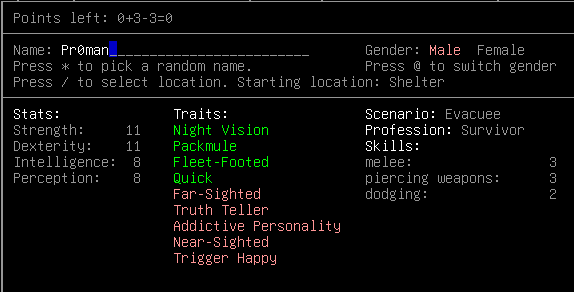
\includegraphics{02}

This would be how our character looks on the finalization screen. So let's hop into the world' is what I'd usually say, but we have some dry stuff regarding the games' story to cover in the next chapter. Don't worry, it's brief.

\chapter{The Story}

The best part of the story? Nobody really knows what's going on (not even the devs). But to give you a quick rundown: You are just another nameless citizen in a near-futuristic (around 2040-ish) New England, a.k.a the USA, when all of a sudden the cataclysm hit and several extra-dimensional beings attack simultaneously. Somehow, you seem to have been spared from the events for the most part and managed to find yourself surviving for the first bit of the aftermath. Now, it's several days after the initial strike and you need to get your ass moving to survive. However, it seems the cataclysm hasn't only brought zombies to the playing field, but otherworldly beings also seem to invade the planet at the same time. This is however not just restricted to one group of beings far beyond our understanding. You are nothing but a microscopic speck trying to survive in a now hostile world, and survive you shall, or not.

\chapter{The Game}
(which you just lost)

Once you pop into the game, you are assaulted by either a weird look of symbols, or a weird look of things barely resembling a crude depiction of the world.

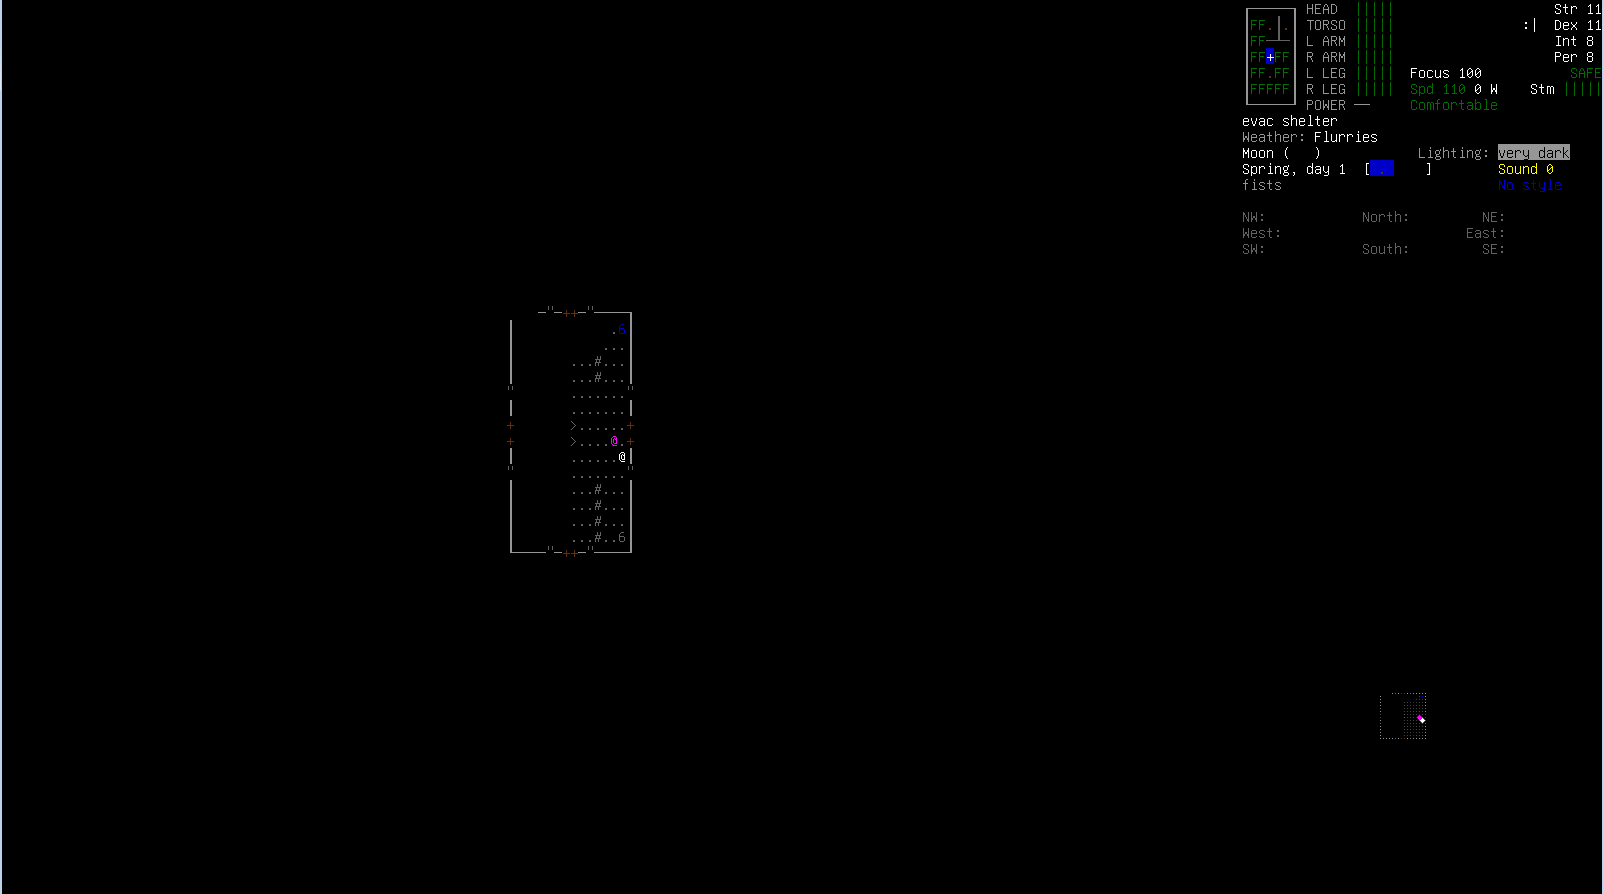
\includegraphics[width=\textwidth]{03}

Woah, who turned off the tileset?

Well, that was me, to give you a general idea of how the game looked in its' original form (which is honestly quite good, especially if you have enough imagination to fill out the blanks, ASCII is something I can always recommend.) if you however press [Esc] to bring up the quick menu, go to Options (or press 2) then cycle to Graphics (lol) using the [TAB] key and scroll down to the "Use Tileset" option, you can and should turn that on. Directly after you can also set up your favorite tileset to be used. I personally use the MSX++LIVE\_PEOPLE Tileset, which is a Fork of MShock, which got forked and improved several times and turned out to be one of the best tilesets so far.

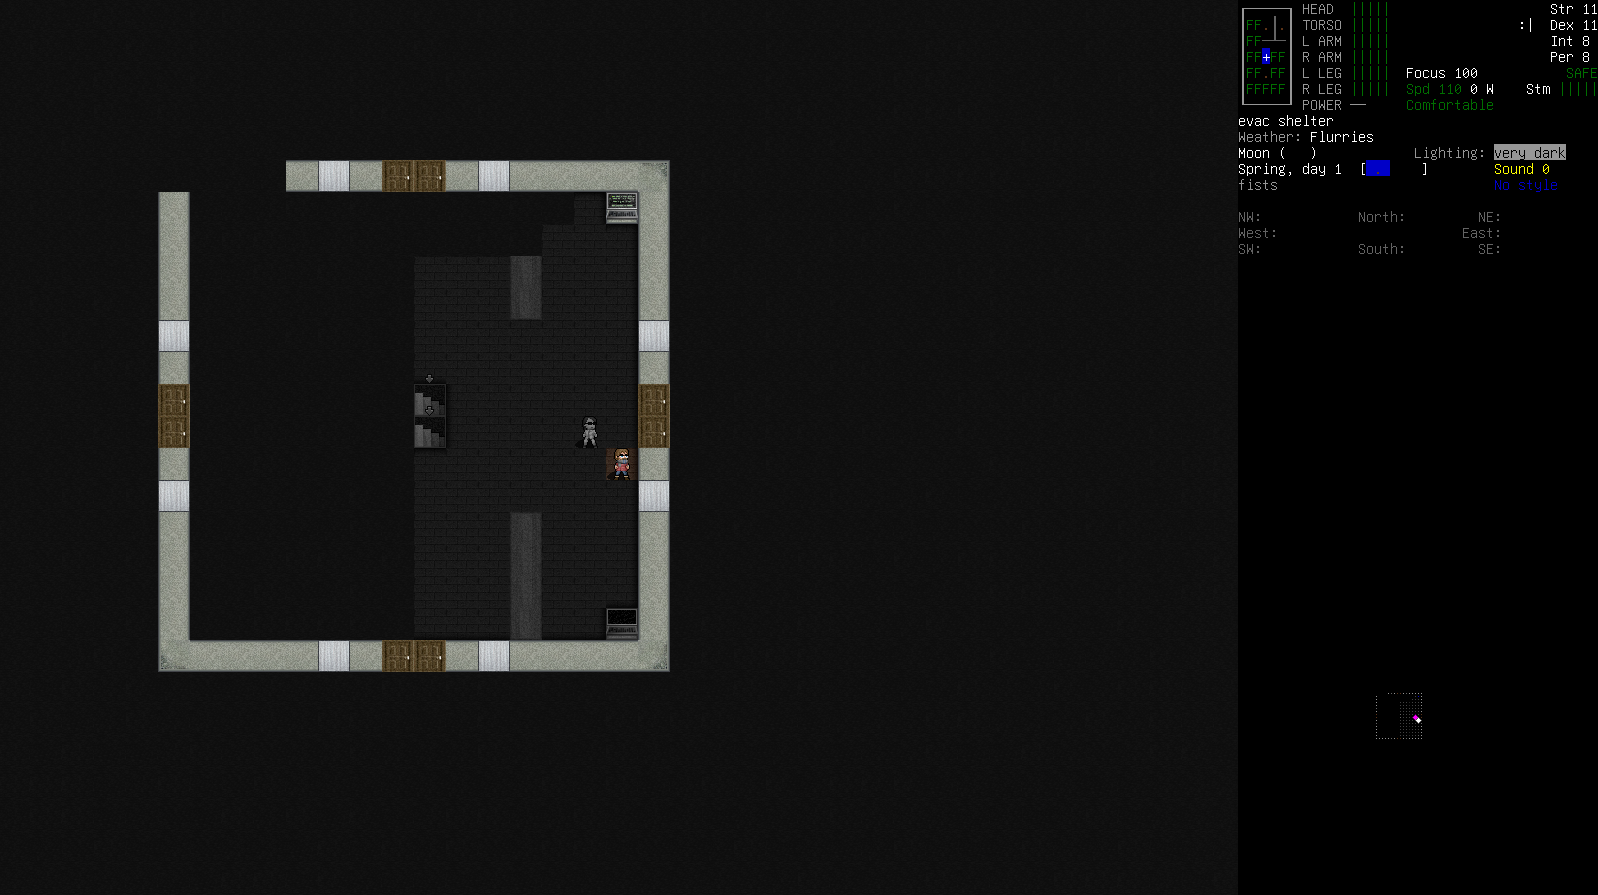
\includegraphics[width=\textwidth]{04}

Ahh, way better, at least you can now determine what's what at a glance. But what's with all that stuff on the left and right side of the game window? The left side might be somewhat self-explanatory, being that you can tell what is located where. On the other hand, the right side seems so cluttered that you are flat-out bombarded with information.

\section{Interface}

(well, that got a rework, but hey, they just moved the stuff around, the contents are still the same)

To get to the Interface that you are now presented with I'm going to use the screenshot again as an example.
The entire left side of the game is your view on the world, what's where, where you are in relation to everything else and so on and so forth, when you issue a command, like a move, this view will slightly change.

On the Right side is the status bar, filled with information that is quite daunting to look at.

At the very top left of it, there is a small 'Overmap Compass', it shows you what the surrounding overmap tiles are, for example roads, forests, houses that come up ahead. Directly below it you can see the name of the tile you are standing upon

To the right of that is your HP, represented as green bars, or if you picked up the Self-aware perk, in numbers.
Wait what? 6 HP Bars to keep track of? Yes, damage done to you in combat is in turn reducing the HP to the attacked body part. This also allows you to see at a glance, what immediate effects your body parts - a red name besides the bar indicates bleeding, blue means a deep wound, green means the body part is infected. If the Health bar changes from numbers to (\~{}\~{}\&\~{}\~{}), it means that the limb is broken and currently not functional.
And directly below is a POWER indicator that only has a bar in it, this is for your current Power to CBMs that are installed into you. As we don't have any CBMs, nothing to see here.
Next up - that empty space in between that and the smiley. Yes, there is something there, you just can't see it. That is where your characters' needs are located. If you feel thirsty, hungry or in dire need of a spot to sleep in, the game will tell you this on that empty spot, even colour coded: yellow means the effect is minor and starts to set in, light red means it is starting to become a real problem and is currently affecting you, dark red means you have a serious issue that could turn out to be lethal in one way or another.

Right below that empty space you see your current amount of focus. This plays an important role in skill gain, but more on that later.

Now for that sweet smiley that looks at you with its' currently more than uninterested look (:|) - this is your general happiness indicator, ranging from (D8 - depressed) all the way to (8D - elated), more on that later when we talk about the mechanics of the game.

On the right of that you can see your Stats, and if they are lowered(red) or boosted(green) by various effects. As we can see, we have 11 Strength, 11 Dexterity, 8 Intelligence, 8 Perception, all things seem to be in order.

Right below the stats you see a fat, green SAFE - this indicates safe mode, a mode that will notify you if something potentially threatening enters your field of view and stopping inputs until you disable it[!] or ignore the monster ['] that caused the alarm. It is a great feature that saved so many players when just doing a walk from A to B without paying much attention, just by enabling safe mode again [!].

Left of that fat green SAFE notifier, you can see some numbers. SPD 110, 0 W and a comfortable in green below that. This gives you an indication of how fast you are. Given our perks, we have a speed of 110% and since we haven't taken a step, walking speed hasn't changed yet.
Comfortable in the apocalypse? well that is going to change, one way or the other. This is just a general indicator on how the temperature outside feels to you with your current amount of clothing on.
Below the location name are currently positioned is the current weather as well as the moons' position. So we know there's some small snowfall going on, and we can't discern the moon's location. Oh well, could be worse.

Right of that is the indicator for light levels: Lighting: Very Dark, meaning we see jack shit as of right now. Why is that? well, all the curtains are closed. Light plays an important role in noticing things and things noticing you (bare a couple monster differences)

Directly below is a calendar, showing the date as well as the season, with an indicator for the suns' position. Since we don't have a watch yet, we can only tell time by looking at the sky, barely.

The yellow sound: 0 to the right of that is an indicator of how loud things are that happen around us. Whenever you take a step, you produce noise depending on some of the gear you are wearing, traits (light step reduces noise noticeably) and/or CBMs and Mutations. Whenever something else in thesurrounding area happens (buildings collapsing, land mines going off), there will also be a bump on that noise indicator there.

The blue 'No style' statement below is showing you what weapon or martial arts style you are currently using. Since we don't own something as fancy as that, we don't use any particular style.

The Directional Indicators - the REALLY important interface panel for the observant survivor. Whenever a monster enters your field of vision, it will be positioned with its' overworld Symbol and its name in one of these indicators, according to its position towards you, obviously.

The big empty space below all of that is a log for messages. How much damage you do, how much damage the enemy does, if you evade an attack, what you just did, everything remotely thinkable off will land in there. By pressing [P] you can access the message log and scroll through recent messages you may have missed.

And last but not least, at the very bottom is a radar that shows you a more detailed look of what you can see. Enemies would be marked as red dots, NPC's as violet dots and so on and so forth. Makes finding minefields somewhat easy if you know their pattern and o
ccurrence positions.

And that pretty much covers the interface, all of those funny values will change when you play, either to the positive or negative, depending on how you do.

\section{Game mechanics}

As cataclysm is a roguelike, it has some mechanics that are inherently difficult to understand for someone who has never touched a game like this before, but even for veterans of the roguelike genre, some of the extra mechanics provided tend to be a bit difficult to wrap your head around. But to give you a general overview on how things are handled on a base level - The game is basically paused forever, unless you do a move. Whenever you perform an action that takes time, everything else performs an action that takes time. This means movement, using items, combat, while things like inspecting what's around you, checking your inventory and the likes do not take time (for whatever reason, maybe you have a photographic memory). So whenever you move, everything else does. You striking an enemy? So does the enemy. All of this is according to the speed of each entity. You have a base speed of 100. Enemies have a base speed according to their internal values (Zombies are usually slow as shit while some wildlife as fast as a road runner). Everything that happens around you is measured in speed relative to you. If you are being slowed down due to pain, poison or whatever, surrounding entities can perform more actions in the time it took you to perform that one action. This can be a pretty annoying effect. While you struggle to swing a slow weapon at the enemy, he can have already performed several hits to you. Which is why it is important to always check your condition. In the following chapters we will talk about the various possible mechanics that you will come across more in-depth.

\subsection{Your Characters' Needs}

Everyone has needs, you do, I do, so why shouldn't your character in a survival game? This is something that you most likely will struggle with in the early game to keep track of, later on it will be more or less just a regular task on your list to tick off. But first and foremost, you should understand what needs you have, how they work and how they can affect you.

So how do your needs work? Every need has an invisible numeric counter in the background ticking down whenever time passes in the game. Once the number goes below a certain point, you will be notified in that blank space to the right of your health, and your stats may be affected. The more pressing a need is, the heavier the impact on your performance.

The big one and I mean the BIG ONE is water. Water is essential for survival, without water, you are a goner within a couple days at best. While being thirsty in itself is not much of a problem, barely reducing your speed (extremely small % amounts), it can add up with other negatives, so having a drink every now and then keeps you happy, and more importantly, keeps you alive. Having a good supply of drinkable water is mandatory for any basic form of survival, besides it being the need that ticks down the fastest, which is also why it is your most important need. Beware, as many sources of water are not inherently drinkable. Most notably - toilet water, which newer players tend to drink without checking the consequences. Drinking unpurified water carries the risk of giving you food poisoning. While ponds and rivers have a chance to poison you, it is in a pinch doable to drink from them to quench your thirst, remember that you are taking a risk. And vomiting out the water and potentially food you had beforehand would just waste supplies as well as hitting your mood badly for a while.

The next big thing on the list is food. Food comes in various shapes, tastes and forms, but it all has one important factor - to keep your stomach filled and you running. Being hungry has no negatives at all, but being famished or worse starts to impact your stats and speed. But rejoice, food is plentiful if you know where to look. Forests have edibles in them for most of the year (Note: Food balance changes made forests way less appealing for their veggies, more for their Nuts and wild game) You can get by eating junk food you looted from houses, off of enemies, but sooner or later, you want to properly stock up on long lasting food.

On the note of finding and eating food found in the wilds - do NOT eat unprocessed food unless you absolutely have to. Eating raw meat carries the risk of catching a food parasite, which are not only unlogged in the games events (meaning you will not be notified), but can also severely hinder any progress until removed by drugs. These hindrances are draining food and water supplies quicker, unexpected pain, messages about your joints aching or hallucinations (depending on what type of parasite you caught). Also, raw veggies usually carry a mood penalty to be eaten raw, so while it works in a pinch, the extra mood drain will quickly stack up and slow further progress for a while, you're therefore better off processing them in one way or another.

And that leaves us with sleep. While sleeping is nice to skip the nights in which you can do only so much unless you have a permanent light source (Which, if you spawned in the shelter, you have in the form of a lit-up Terminal) it is also essential to not suffer sleep deprivation. While it is the need that is the least necessary, it still is a necessity, simply because being dead tired imposes a great hit on intelligence (-4) and therefore makes crafting way less efficient. To go to sleep, hit the [\S] button and select that you want to go to sleep. You can sleep anywhere, from the concrete of the road, to a bed or in a vehicles' seat. Each on its own having a certain difficulty to fall asleep on. Sleeping on a hard floor is obviously way more difficult than sleeping on a bed, but even if that is not a possibility, a bench or table is better than sleeping on the floor. There are also items that assist you in falling asleep, like pillows. Just have them on the tile you wish to fall asleep in. Remember though, that you just don't fall asleep the instant you lie down, and being sated and full, having a proper bed (or seat) to sleep in, as well as actually requiring sleep makes it all the easier to fall asleep. Make sure to go to bed early and potentially wake up earlier, as waking up late means you wasted precious sunlight in which you could explore, craft and loot.

While not technically a need, you will quickly perceive it as such: Your happiness, or in other terms - the mood.

Mood is an interesting thing to take notes from: If you are unhappy with life, you definitely will feel the negatives, while being happy seems to have little effect on your day to day life. But how does it actually manifest its' negatives? Well, for once, you will be slower in crafting or straight out refuse to do work (this includes vehicular work and butchering/disassembly), however, your skills will also be affected, though in a different way - you will gain experience much, MUCH slower than normal. How come?

You remember that smiley as well as your Focus points? Those now come back into the talk. Your mood, at a quick glance, is depicted by that smileys expression and colour, red meaning bad, green being good, totally fine so far. Your mood (viewable with [v]) will also list your current focus point gain/loss per minute. Being unhappy drains focus, being happy refills it quicker. But what is focus? In simple terms - it's unspent experience. You spend this experience by performing actions that would gain you experience in a respective skill whilst draining from the pool of focus. So the more focus you have, the better you are off to train skills, either by reading or by doing the actual related tasks.

So what should you aim for on your focus? The higher the better obviously. But, what is the normal value of focus? For any character without any particular mood effects, it tends to fluctuate around 100, depending on actions done. High mood increases this to 130 somewhat easily, with some dedication and work put into it, values of 160+ are achievable. But this can also turn the other way and you can easily end up with being stuck at 30 focus, either by draining it heavily - combat is a great way to do so - or by doing bad things. But what could be considered bad in a world where there's the living dead and extraterrestrial beings roaming the world? Well, your character is still a human, and may think of human life as valuable. Killing other humans can occur a hefty penalty (killed innocent: -100 happiness), as can losing a friend (long-term companions that you recruited using the 'We're friends' talk option, as you will also consider them a friend, just as they do you). This is not the only threat to your happiness, as things that one would have scruples killing, like zombie children, will occur a small, but stacking penalty to your overall happiness. However, the biggest threat that you can encounter in this regard is not the undead, not the humans (those are too rare anyways to be a bother), but rain!

Being wet, which your clothing most likely will not protect you from, will incur a nasty -55 penalty to your happiness and also carries the extra risk of you catching a cold. While it is absurdly easy to remove (use a towel), you can quickly forget that this is an option.

Another interesting 'need' that may or may not pop up is the need for certain addictive substances. If you started as a character that is currently addicted or you consume too many items of an addiction category too quickly, you soon run the risk of becoming an addict.

Addictions are outright bad. Being addicted can, depending on severity and type of addiction, cripple you for several days or weeks. But how do you actually obtain an addiction?

Every player has a value of 0 for each addiction type - Whenever you consume a drug that has an addictive quality to it, it has a chance of increasing that value by 1 (for each type respectively), this chance is based inside the code for each item. Caffeine is way less addicting than Crack obviously. Once you hit a value of 3, you are considered addicted and will start to suffer the effects if you are craving for that particular substance.

So, how do addiction play out? Whenever you feel a craving, you will suffer negative effects. You may either wish to just ignore it, or take the drug again to sate your needs. When you decide to take a drug, remember that it has a chance to increase your addiction value. Doing so, however, will set an internal 'sated' counter to 1200 (800 for addictive personalities), decreasing each 100 time units, or generally speaking each turn, by 1. Once this counter hits 0, or goes into the negative, you will feel the need for said drug again.
Once you reach a sated counter of 0 - addiction level * 100, your addiction level will be reduced (used to be halved, but changes to the system made going cold turkey take quite the bit longer, now it is almost linear). Note that higher levels of addiction will have more severe effects than just starting to become addicted.

But what negatives are there? These are dependant on each addiction respectively, but more often than not, these effects include morale penalties - depending on addiction type around -50 to -250, reduced Stats, induced nausea, giving you pain, having hallucinations or effects like the shakes popping up.

So drugs aren't inherently bad kids. Just make sure to use them appropriately and sparingly, not liberally. Especially now in the apocalypse, in which your best way of obtaining drugs is to either luck out and find them, or make them on your own. Their respective effects may save your life at some point.


\subsection{Temperature and Clothing}

While each topic on its own could deserve an entire in-depth chapter to it, I decided to put them together, as they are closely connected.

First of all, we will talk about temperature. Every location has a temperature depending on the overall outside temperature and it's insulation. Having open windows in a house will decrease the temperature inside, having a fire inside a house will increase it, pretty standard so far. Outside is usually the coldest (bare one specific overworld special) while some tiles generate heat on their own, like fire or lava. Why does this matter? Because temperature has its effects on you. Being cold ,which changes your temperature indicator from a green 'comfortable'(falling) to a light blue 'chilly' or even worse depending on how cold it actually is, has detrimental effects to your speed. The colder you are, the slower you are, and as we talked previously, being slow means everything around you is relatively faster now, being able to catch up, getting in hits more often and so on and so forth. Not only that, but if your body parts get too cold (yes, temperature is checked for each body part), it'll start to slowly take damage, more so if it gets even colder. This can quickly kill any undergeared character who is stranded out in the wild. The other side of the spectrum isn't much better though. Being warm also slows you down, though not nearly as heavily as being cold. Being hot drains more liquid than usual and being close to various heat sources (fire, lava) also can damage your body parts. Dropping into the very hot! temperature range will put you into the famished food requirement via vomiting and therefore can severely cripple you. So being either too hot or too cold can be detrimental to your health. How do you take on cold temperatures then?

Well'

Clothing is the answer.

Clothing has several different 'attributes' as we will call it here, that define their values for Survival as well as their potential usefulness in certain situations. It should be noted that there is little in terms of limitation when it comes to clothes. You can wear as many pieces as you like, but never more than 2 of the same item. So you can totally wear 2 Backpacks, 2 Duffel Bags, 2 Makeshift slings, but never 3 of them at the same time. This limitation does also apply to Helmets and Boots in particular, as you can only wear 1 piece of Headgear and 1 Pair of footwear.
Nevertheless, let's take it from the top, you could say each piece of clothing has the following attributes:

-Body part(s) it is worn on
-warmth provided to that body part
-\%-Coverage of the body part(s)
-Layer it is worn on
-encumbrance to body part(s)
-armor values provided to equipped-on body part(s)
-material
-additional modifiers

So, now to take a look at these attributes.

The body part(s) a piece of clothing is worn on - this is pretty self explanatory. If you wear something that would cover your entire body, say, a suit, it will cover the appropriate parts, namely the torso, arms and legs. A bandana for example will cover your mouth. You get the idea, You can also just check the items details to see what body parts it covers, as well as'

-Every piece of clothing comes with a warmth value to it that it will apply to the body part that it is worn on. If your clothing piece covers multiple body parts this value is applied to each body piece at the full value. On the note of that, most of the clothing follows logical values when it comes to its' material. Fur is, for the amount of material used, warmer than leather, which in turn is warmer than cloth.

The \% coverage of the body parts it is worn on - The effect of which is really important.
The potentially most important effect later down the line is the effect it has on armor values applying. Think of it like this - If you have a piece of clothing that would provide you with 20 CUT and BASH armor, but has 50\% coverage, that basically means that half the attacks have to be calculated against this armor value, while the other half goes past it unhindered. Makes you look at that piece of clothing a bit more carefully right? With all of that in mind, how are you ever gonna survive in your street threads considering they only provide so much warmth and only cover up so much? Well, this is where'

Layers come in handy - each piece of clothing is not only assigned to a body part, but also to a layer it is worn upon.
There are 4 layers (technically 5)on a body part: Close - belted - Normal - Outer - Strapped

To quickly clarify - belted, or rather 'worn around your waist', as it is called in the game, refers to, well, belts and tools that can be worn on belts via loops. Considering tool belts and the likes are therefore unique to the rule of clothing when it comes to their layering, as they can only ever cover one layer, I just wanted to mention it since you hardly come across a reason to wear more than 1 belt, as they only have so many uses.

Without suffering penalties, you can wear 1 piece of clothing on each layer for each body part. What the layers do to you specifically is pretty simple - for warmth, they add up all the warmth values to that body part. So while outside temperatures could be at a rating of -20 (temperature for the character's feelings' sake is measured on a range, while temperature also exists as a proper scaled unit in Fahrenheit or Celsius, right now, the rating matters) for a naked character, having clothing on each layer with a warmth of 10 (and for the sake of simplicity, 100\% coverage) would put you at a +20 rating, which is pretty comfortable. Going over this would be considered warm, hot etc.
On the note of high temperatures it should be stated that there is no way to reduce the ambient temperature. While you might think that this is not that big of a deal, since, hell, when are you ever gonna be close to a fire, remember that in order to reduce the felt temperature, you have to unequip gear and you only wear so much. If you were to stand close to a burning building for example, all the different Fire tiles generate lots of heat. While this seems minor, the effect that this can have on you can be extreme. There are no limits on how cold or hot an area can be, with several fire tiles stuck close to each other, being near a burning building can quickly raise your felt temperature to a point that will endanger your life, as hot temperatures can have just as negative an effect on speed as cold ones, while also damaging your affected body parts. Sooner rather than later you will have the feelings down for how much clothing you require in the appropriate seasons as well as day times. Usually, the more is better, except for the clothings' negatives'

Encumbrance, or how difficult it is to move in your clothing. Again, layering helps, as you are suffering no penalties for wearing 1 piece of clothing for each layer of a body part. Each piece of clothing makes movement more difficult in a certain way, as each body part has a different negative while being encumbered:
Head:
-does currently nothing and only limits what you can wear (to not stack helmet after helmet on your head)

Eyes:
-negative 1 Per while checking traps for each 10 encumberment
-Extra +0.5 throwing dispersion per point of encumbrance
-extra +0.25 ranged dispersion per point of encumbrance

Mouth:
-running costs + (mouth encumberment lvl * 5) increased stamina
-decreases yelling volume

Torso:
-negative 1\% melee to hit per point of encumbrance
-melee swings cost +1 movement point per encumbrance
-negative 0.1 dodge skill per point of encumbrance
-swimming Encumbrance Lvl /10 * (80 - Swimming Skill Lvl * 3)

Arms:
-extra aiming penalty by 2*arm encumberment

Hands:
-extra reloading time: 30*hand encumberment lvl
-throwing dexterity (throwing - hand encumberment lvl)

legs:
-Running cost + (leg encumbrance * 3)
-swimming cost: encumbrance * (50 - Swimming Skill lvl * 2)
-dodge skill: -encumberment/2

Feet:
-running cost + (feet encumbrance Level * 5)

Basically - the more you wear, the less freely you can move, which, in combat, can be pretty hampering. However, clothing does make up for it, we already know that it has warmth, we know it's protecting you, to a degree, but how does that actually work? We'll talk about that now:

Armor values on gear are what is between you and the zombie that is trying to maul you and use your skull as a muesli bowl. Armor is separated into the following damage types: CUT, BASH, ACID, FIRE, ENVIRONMENTAL. The more it has, the better protected the body part is, makes sense right?

Yes and no, again, coverage is king on the matter of BASH and CUT. Since \%-Coverage determines if a hit done to you will be reduced by your respective armor values, or bypassing it in its entirety. This will be checked for each layer that you wear when a body part is attacked. So it may be worthwhile to stack up on as much armor as possible for each body part, right? No, have you not payed attention yet? Armor that is fully covering and has great protective values will most likely encumber you to hell and back, making you nothing short of a sitting duck, ready to be ripped apart. It is a fine balancing line that you need to find for yourself, how many pieces of armor and clothing you require to not be too encumbered whilst also being protected enough to not just straight-up get killed in close combat.

But what about the other values? Well, Acid protection means that you are able to withstand attacks that would be considered corrosive and that will deal relatively quick damage to the hit body part. You will quickly, and potentially painfully learn to avoid these kinds of attacks once you get into actual contact with them while unprotected. But how does it actually work?

Values in the Category for ACID give you a resistance to being affected by hit acidic attacks. To be able to stand in a pool of acid (not that you'd willingly want to), you would require a flat 5 acid protection on your feet and legs to withstand the acid damage from standing inside a field, yet this doesn't make you impervious to standing in the acid field idle, 5 protection only makes you partially immune, though you do take substantially less damage from it.
Your legs? yes, you only have 6 body parts, 4 extremities, a head and the torso that everything is attached to, so feet and hands are considered to be legs and arms respectively.

Now, what about fire? Well, any gear that is flame-resistant (Basically created out of Nomex) will not only douse you quickly if you managed to get set ablaze, but also reduces the damage to the covered body parts substantially, making it possible to survive a trip into fire. Just don't expect to be surviving for extended periods of time.
As a note on certain materials, clothing that is made out of either cloth, leather, fur or wool will catch on fire and take damage until the fire is put out, or the item in question destroyed.

Environmental Protection? Well, this is something special that I feel should be explained more thoroughly. It will basically allow you to potentially ignore certain field-effects and stop you from catching diseases (if you wear enough mouth protection, that is).

Those field effects are (just to name a few): sludge, acid, electricity, gas of various kinds, webs etc.

As you can see - acid is on the list, so you also require environmental protection as well as acid protection to gain potential immunity, tough this would usually be nothing to work towards on the first couple days, it is something to keep in mind later down the line.
So how does it work?
Well, whenever you would happen to be affected by a field-effect, the game checks its' strength against the strength of your environmental protection for the affected body part.

But there's still 2 attributes to name - so let's go over the material that your clothing is made out of: While the material seems to have little implications on how a piece of gear holds up (leather armor can be nearly as good as a kevlar vest, it all depends on how it's made obviously) when faced in combat, it is the defining factor in repairs. You can use your tailoring tool of choice to fix clothing worn or in your inventory, and whatever material it is made out of is required to do repairs. Not only that, but it dictates the tools applicable as well as the skill used. Items that are worn, yet require fabrications to be made, check against the fabrication skill and more often than not (considering most fabricated things are made out of metals or plastic) require different tools, like a welder or soldering iron instead of a needle or sewing kit.
To go into more technical details about material effects - each material has its own values for defence assigned in the games' files. Each piece of clothing has its own material thickness (which you can't see) assigned to it, this in turn assigns how much protection a certain piece of clothing offers. So in general terms, something made out of Kevlar is generally better than something made out of Leather, except for the fact that the clothing thickness could be higher and therefore superior, but it is a general rule of thumb that does apply.

And last but not least, each piece of clothing can have several extra effects, which I'm going to list:
-pockets
-hood
-rain protection
-gas protection
-radiation protection
-electricity protection
-built-in sheath/holster
-tool storage/loops
-durability (not exclusive to clothes, but is still a special)

Well, what do these do?
The built in sheath as well as the tool storage seem obvious - [a]ctivate the piece of clothing to store an item that can fit into it. It still counts towards the tools you are carrying if you do certain tasks, like a sheathed hunting knife still being able to butcher corpses, or a hammer being stored in a toolbelt if you were to deconstruct furniture.

The pockets are self-explanatory in their description, as long as your hands are free (you not wielding a weapon), you will use those to keep your hands warm.

The hood will be used in the same way, as long as you are not wearing headgear (a.k.a your head is unencumbered)

The Protection from rain reduces your overall penalty for being wet for each body part that is covered. So if you were to get gear that completely covers you and had this effect, you wouldn't feel the effects of rain at all.

Gas Protection is pretty much exclusive to suits in their entirety and Masks, like Gas/Filter/ABC/PBM Masks. Those will require cartridges, as whenever they filter harmful materials, their charge will drain by 1. Make sure to prepare them before heading into battle on gas tiles though, as the preparation delay may cause you to inhale gas before it is too late. Don't worry, charges will only by drained while actively protecting you.

Radiation Protection as well is being exclusive to suits, mostly things like Hazard and Clean suits, these will shield you from any outside radiation. However, if a monster attacks you that would carry over a radiation effect, this will bypass the suit (mostly comes from mods)

Electricity Protection also comes from suits, most notably, the Faraday suit, which will protect you from arcs of lightning zapping you as the suit will be grounded. However, this does not apply to zapback by attacking something conductive (like a shocker) with a weapon that will conduct electricity or your bare hands.

\subsection{Crafting}
Time to talk about the single-most important aspect of the game - crafting.
You wouldn't believe how much code is reserved for crafting alone, especially when you consider that you can also pretty much disassemble whatever you think off. But how does it actually work and what benefits do you, as a survivor, have from it?
To take it from the top, it works by opening up the crafting menu [\&] and being again bombarded with recipes, sitting in categories and subcategories and the list goes on and on.. But not to be intimidated by it, all crafting procedures follow the same steps you need to fulfill to be allowed to craft an item:
You require the appropriate tools (some also require charges)
The appropriate components to make said item
Time, obviously, you won't just create an item in the fracture of a second. (most of the time)
And, optionally, light. If you can't see, you can't craft.

First of all, we need to navigate this place though: [TAB] and [Shift] + [TAB] to navigate the top selectors, [<] and [>] to navigate the subcategories and the arrow keys or NumPad inputs to scroll around inside.
If you however want to look for a specific item, you can also open up the search by pressing [f] inside the crafting menu. You will be shown a bunch of search parameters you can look after. This is a godsend, as it quickly allows you to search for items with the appropriate qualities, what something might be a component out of to guess its' value and so on and so forth. If you have a search results page opened, press [r] to clean the results and head back to the standard crafting overview.

As of the recent versions, the crafting window has been given a new Tab - the Recent/favorite items menu. If you see yourself using certain crafting recipes, but are not interested in searching them all the time, you can just quickly mark them as favorite in order for them to appear in this quicklist instead of you having to search for them each time you wish to craft something. The 'recent' subcategory will memorize the last crafts you have done so you can quickly access these recipes there as well.

Should you notice that you are unable to craft a certain item despite you having all the components, make sure to check if all the conditions are met - is it bright enough or are you too sad to perform a craft? The Top right corner will tell you in red what the issue is. Is one of the tools marked in a brown color? That means the Tool property is on an item that is also a component of the craft. You can't just hammer a rock using itself into pebbles, nor can you use one of your two makeshift welders to turn them into a vehicle welding rig - you require an extra tool that provides you with that quality.

But why is it such an important factor in this game? Well, from boiling water to making powerful firearms with their respective ammo or tailoring clothing, everything that is done via the [\&]-menu is considered a craft, and this is how you, for example, also prepare your food and turn it edible. Not only that, but the devs seem to have thought of so many variables that it's mind-boggling. Forget Fallout 4's scrapping system, this is where it's at. You require a flashlight? No problem, a lightstrip or light bulb, some scrap metal, can or similar container along with some copper wire and an amplifier circuit and voil', one flashlight (without batteries though). And if you were to deconstruct it, you will also receive these same items you were using in that craft. So if you accidentally crafted your last power converter into an item you didn't actually intend to craft, or required that for something else, you might be lucky in that you can deconstruct it. Not everything is deconstructable, as this requires a lot of attention to also include in the code, though the devs have made the effort to include deconstruction - recipes to most items in post, where it makes sense obviously. Items can be deconstructed in the following ways.
open up your inventory, select the appropriate item and select the 'Disassemble' option.
if the item is on the floor, move onto that tile and press [B] to open up the butchery menu, items that can be disassembled will have a selection with a capital letter and only their name next to it. If you wish to scrap an item, you can 'cut it up', however, this will most likely not return all the items and instead scrap resources will be gained.
Use the disassembly menu [(] to select items to disassemble quickly from your inventory or the nearby ground (the 8 tiles around you)

What do you gain from that, apart from the satisfaction of creating that item you want? Well, for once, experience in that respective skill. Crafting things that require the skill electronics increases that, crafting fabrication items increases fabrications and so on. However, there's also the other side of the coin - you can fail on a crafting operation, with different severities.
When you craft, each recipe has its' own difficulty, determined by the skills required and if you meet these and your intelligence (which is weighted against this). If the skill required of the recipe ties with your actual skill, there is a small chance of failing either without using materials ('white fail') or with wasting all the materials required ('red fail'). If you don't fulfill the skill requirements for a certain craft, yet are able to do it because you own a book that contains this recipe to use as a reference, or a follower NPC know the recipe and therefore can also provide you with it, this effect is even more drastic and you will most likely fail. If your skill is substantially higher than the required skill for a certain craft, you will also gain no experience (after several crafts, you will receive a notification in the message log about those tasks being trivial)

On the note of crafting and their respective tools - Tools will never be consumed upon a craft unless they are also part of the components required (the bottom list of items), not while failing or succeeding. HOWEVER - red fails will drain charges from your tools (if applicable)

\subsection{Construction}

Construction pretty much works the same way crafting does, for the most part, and is accessed using the [*] button. It will bring up a list in which you can filter and search, by pressing [f]. Each construction has several requirements:
The appropriate tools
The required Materials
The skill required for it
and a space in which you can build it.
Light is interestingly enough not relevant for doing construction works.

But why would you bother constructing things if there's structures all around the world, ready for the taking? Well, walls can be damaged or broken in their entirety, requiring some makeshift fixing or replacing. You might want to board up windows or doors early in your career to limit visibility as well as entry points for zombies (though they can bash through if they run into it or notice you on the other side). Some tools and stations might help you in your craft, most notably the smoking rack for food preservation or a rock forge for smithing items. Or you just want to dig something resembling a moat by digging deep pits around your base to deal damage to incoming zombies, which are more than willing to step into it (this can be used to create trap areas). So there is more than enough applications for doing it, it all comes down to what you want to do and how much you are willing to invest into a certain location.

\subsection{Combat}

The big challenge when it comes to new players - combat, or 'WHY AM I DYING AGAIN ALREADY OH GOD MY ARMS ARE GONE'.
Combat, while simple to perform, can quickly confuse players with its' many factors and quickly leave them dumbfounded and dead when they were so certain that they could beat the enemy. This is why I wish to make an explanation as to what is happening:

Whenever you were to move into a tile where an entity that is either neutral, or hostile is located you will perform an attack towards that target. It will cost you a fixed amount of movement points according to your encumbrance as well as the weapons speed (encumbrance effects are a flat addition to the speed of a weapon).
Once you do issue the command, you will roll with a x-sided die to check against the enemies defences. Here come all your skills into effect - weapon skills, melee skill as well as the to-hit bonus of your weapon, which flat-out adds (or subtracts if it has - to hit) sides to that die. The die the enemy rolls is sided based on their defensive skills as well as their size (citation needed) and if you manage to surpass the enemy roll, you land the hit.
Same goes for the enemy - if his die, which is affected by the internal melee skill the enemy is given- will surpass your defensive roll (which is decided by your dodge skill modified by your equipped gear) he will land a hit on a randomly targeted body part.
But how much damage does he do? Well, each monster in the game is given a certain damage value, determined by dice with the appropriate amount of sides + a flat damage value, a damage type, and an armor penetration value. So lets say a monster could have cutting damage, 0 armor penetration and 6 dice with 6 sides, as well as +10 damage, this would mean at minimum he would deal 16 CUT damage with a hit (10 flat + 6*1 roll) or at best (for him, not you in this case) he could deal 46 CUT damage (10 flat + 6*6 roll).
This end damage value will then have to pass the armor check. If you wear something on the targeted body part that has 20 CUT armor (we ignore BASH for this real quick) and 75% coverage, this would mean the enemy has a 25% chance to bypass the armor value and hit for the full amount of the roll. If he would fail the check, however, the damage value would be subtracted by the appropriate armor value.
So for a hit of 16 damage (the minimum) you would take 0 damage in this case('The enemy hits your [body part] but fails to penetrate armor!'), or you could take a nasty hit of 26 damage -if his damage roll had the maximum damage to it- to said body part, which not only reduces your HP, but also induces pain. Quite severe one at that point. The more HP you lose, the more pain builds up, slowing you down, reducing attributes and so on. So it is difficult to swing back from a fight you are losing simply by luck. If you are winning a fight, you will just 'win more' and the enemy usually won't pull out a fancy magic trick to change the tides' more often than not.
Later game enemies can have special attacks that induce status effects or deal tremendous amounts of damage, so be sure you know what fight you are picking.
But what about pain? Well, it's the reason people die. Not loss of HP, but pain usually is what loses you a fair fight. Damage dealt to you has a certain pain buildup that will increase the current felt pain by a certain amount. Pain is long-lasting and without the help of painkillers, will only reduce slowly over time, but what effects does pain have?
Well, the higher your pain, the slower you are - this is the most obvious effect and also the most brutal to deal with. As you may or may not remember - the slower you are, the faster things around you are (relatively speaking), allowing them to get more hits in. Not only that, but pain also reduces your stats, not too badly early on (very small amounts of pain only reduce Int by -1) but quickly adds up so you can lose heavy amounts in all stats, most notably - Str and Dex, at high Pain levels -3 to 4. And as we know, Str and Dex are defining combat stats. This means that your melee-dice will suffer by getting into heavy amounts of pain, which not only reduces your hit-rate already, but worse yet, pain also reduces your hit chance by a certain amount directly ('Your pain distracts you!'). So, the heavier the pain, the more you are fucked. You can counteract this by popping in painkillers (Aspirin, Codeine, Morphine, Tramadol or homebrew stuff like Poppy Painkillers), this however - depending on how strong the stuff is you just threw into your system - can also have negative outcomes when it comes to your stats. Not just that, but painkillers require a time to kick in properly and only reduce pain by so much, and worse yet, they can be addictive. And if you call now - more nasties - you can overdose on Painkillers and die due to asphyxiation (a Painkiller value of [50]+).

Well, that was a bit of a sidetrack, but a noteworthy addition since it is an important part to keep in mind, since pain dictates the flow of combat and how you might want to behave in the next couple of turns. But what about when you attack something? How does your damage calculate?

Each weapon has its own damage type: CUT, BASH or PIERCE (technically that is also cut with a different flag to it)
and other factors that all should calculate into if you want to use a weapon or not, but let's not worry about that, as we will just assume you landed a hit. The weapons damage values (which you can see by checking it in the inventory), as well as your Str damage bonus (visible in the [@] screen) will be added together to your melee dice roll(which will increase with more melee skill at high levels)(citation needed here) and determine the damage done to the enemy minus its armor values. Each enemy has a fixed amount of armor for different damage types - CUT and BASH, as those are the only 2 damage types a player can do. PIERCE is a derivative of CUT and checks against this armor type. Bullets and the likes tend to go for CUT damage (except for blunt ammo, like target arrows, or Beanbag rounds which deal BASH, or piercing ammo like Flechette which also comes with heavy armor-piercing values).

Each strike done against an enemy will, however also have the chance of being a critical hit. This has the added benefit of being maximum applicable damage and your chance to land a critical strike increase with the appropriate weapon skill.

But what about that fun little green bar called stamina? Well, each weapon has a fixed stamina cost to swing. Each movement done has a fixed stamina cost - usually not noteworthy, unless you are overburdened, which increases the cost the higher you are over your limit or when your legs/feet are too heavily encumbered, most likely a combination of both - But we will only worry about the swing. Stamina required for a swing is based on the items' weight and volume and therefore speed - swinging a knife is definitely easier than swinging around a 100L wooden barrel. The stamina cost of your swing will also be modified by the current encumbrance to Torso and Arms. so be sure to not be too heavily wrapped up in gear. Why does it matter? Once you run out of stamina, your swings will hit for less and take up lots of time, not to mention the winded effect, which occurs when you drain the entirety of your stamina and need to catch your breath (-4 all Stats). But swinging fast and for little cost also comes at its' own risk - if you deal next to no damage, you are gonna be winded in no time regardless. This is most notable when doing unarmed combat and also the reason why it is a quick and easy way to get hurt. While unarmed combat is great for murdering zombies once you hit a decent level (3 is minimum for most players, 5+ recommended), when just starting out at rank 0, you will most likely hit like a wet noodle and just waste stamina. So even something as simple as stamina management can be a win or loss determining effect in combat.

This however is most of the things that I can cover in the topic of combat, so we should move on.

\subsection{Status Effects}

While being in combat is no fun - or maybe it is, you masochistic survivor - there's more side-variables you need to pay attention to, not just in combat, but in general. Status effects are ailments inflicted upon you because you stepped into a tile that landed a field effect, got hit with an attack that carries over a status effect, or because of you being unlucky and getting hit by a disease (those are also considered status effects). The variety of effects is great and you aren't supposed to learn them all by heart, but it is something to keep in mind, either when gauging to take that fight or not or what to resolve when moving forward.
Status effects trigger certain events with a certain frequency - what does it mean?
Let's assume you inhaled a lungful of smoke. This is the status effect. It will cause you to cough, which costs you stamina and makes noise - this is its event. You will be coughing at a very quick pace - this is obviously the frequency. So now you are having to wait out its effect, sitting there, coughing - draining stamina, and once you are out of stamina, damaging your Torso HP until the status effect wears off.
This is how status effects work, effect - events - frequency. There is a bunch of status effects that one should be aware off, however, if you ever feel like wanting to know how affected you are, press the [@]-button to see the general character overview and switch over to the current effects window. There you can see which effect does what and how often it does it. Beware that some effects, like parasites, are not listed here. Some status effects you should know about are:
Poisoned/Badly Poisoned - not only deals damage and is considered a painkiller, but slows you down drastically
Painkiller/Stimulant overdose - Occurs once the Value for either Painkiller or Stimulant hits [25], impacting your stats heavily.
Bite wound - If you take a hit from a bite attack during combat that manages to penetrate your armor, there is a chance of you receiving a bite wound. This wound will cause pain over the course of its existence and has the chance to turn into an infection that will inevitably kill you later down the line if left untreated. Treat such wounds using antiseptic items (antiseptic liquid/powder, hydrogen peroxide) or if those are not available, throw some Atryupan into your system and hope for the wound not getting infected, or just pray to whatever higher being you believe in that your health stat is strong enough to not turn the wound infected, as each player has a base chance to not carry an infection and the wound clearing itself after a sufficient amount of time.
And if you manage to not do so or get unlucky, you end up with an'
Infection - This is a serious problem that could end your run. You only have 24 hours from the moment the wound turns infected to being treated by using proper Antibiotics. Not just that, but while you are infected, your stats are severely hampered (-2 each, increasing in severity over the course of the infection) And once the infection progresses far enough, you'll randomly pass out, which is the last thing you want in such a situation.
You could also be extremely lucky and hope for an infection to cure itself, however, a freshly spawned survivor with normal health stat has only an all around 10% chance of surviving the infection, around 25% if you picked the 'infection resistant' perk.
Adrenaline Rush - Boost to Str, Dex and Per at the cost of Int (-8), constantly regenerate Stamina and speed boost.
Adrenaline Comedown - speed debuff (-10%) and Stat reduction (-2 each)
Having a Smoke - +1 Int and Per
The Shakes - This is usually a craving effect caused by addiction, but can also happen due to the trait 'Jittery', which is pretty much the opposite of an adrenaline rush - your dexterity will be hampered at random while under stress or under the effect of Stimulants. (-4, also -1Str)
Radiation [x] - with x representing the number, your radiation level can have no consequences at all, positive benefits or (for the most part) negatives attached to it. Being irradiated with 1 or 2 points is hardly noticeable, with it slowing you down by only a small percentage amount. Yet, hitting radiation levels of 5 and upwards is where it becomes an immediate Problem that requires fixing. At 5+ you will randomly become nauseous, which in turn could lead you throwing up all the tasty potato chips you just downed, turning the positive mood into a hefty negative. Being irradiated at all also damages your health stat (more on that on the next chapter) while also slowing down your healing naturally and at ranks 10 upwards you will start to take damage to your entire body. Not only that, whenever radiation ticks down, there is a chance of it eating a whole lot of radiation ranks at the cost of obtaining a random mutation, the more irradiated you are, the more likely it is, if the radiation itself won't kill you. So what benefits are there, except you may be glowing in the dark soon? Well, specific perks can work great in combination with high ranks of radiation - Most notably Robust Genetics. If you are willing to gain random mutations, this is a cheap way to just mutating without too many negatives, though you will gain mutations of all different kinds, some may be undesirable despite being labeled as 'neutral' or 'positive'. Another great perk is Radiogenic, which slowly heals you while you are under the effect of Radiation. But for the most part, avoid radiation at all costs and if you have to stay in a radiated area, make the trip short, or pop in some potassium iodine.
Hungry, Thirsty and tired are also listed under the general effects window as status effects with their current level of incapacitation to you.
You should make it a constant habit to check your general overview screen [@] after combat or when visiting certain areas to see if anything special is affecting you, but this pretty much covers all there is to some of the more notable status effects, so we shall move on.

\subsection{HP and Health}

Alright, the big thing that takes up a bunch of your interface, as well as being the determining factor of you either biting the bucket or making it past a hostile encounter. Let's talk about HP first. According to your Str value and the base +60 HP each body part has on its' own, you will have a maximum HP value for each of your body parts, usually somewhere around 80-92, besides that, the interface allows you to quickly tell in what condition a limb is: a red name means you are currently bleeding, a blue name means the body part has a bite wound, green means that body part is infected. Or, if the HP bar looks like this (\~{}\~{}\&\~{}\~{}) it means the respective limb is broken and unusable.
Taking damage from various sources will decrease your HP, while sleeping, having some specific perks, or having a treatment applied will restore HP to you. Pretty standard, but how is it determined how much HP you get? This is in turn decided by your health stat, which is usually hidden (exception being the self-aware perk) and has a base value of 0 and can range from -200 to +200. Being positively healthy means you will heal faster, your limbs mend faster and you will have an easier time fighting off diseases, bite wounds and infections. Being in the negative has the opposite effect, you heal slower (or not at all at -200 health), you will catch diseases more often, fighting off bite wounds is gonna be harder and infections will most of the time be lethal (not like they are already). How do you gain health then and not lose it? Well, health always tries to move towards the middle point, 0, so if you are in the positive, you'll lose health by time passing while on the other hand if you are in the negative, it'll slowly gain towards 0. But you can supplement this by eating healthy foods most notably. Foods found in the wild generally have a positive health value attached to them, as do several later cooking recipes that employ multiple components. For a quick boost in health you could also just pop in a gamma-globulin shot randomly found in households or medical buildings. On the other hand, losing health is surprisingly easy - taking damage, being radiated, eating unhealthy food items all reduce your health rather quickly and start to pile up on the effects of you being slower to heal to peak performance. There are also CBMs, positive and negative, that will affect your health stat. A botched installation can install a leaky bionic, which will constantly eat away at your health stat until you bottom out at -200, while the leucocyte breeder CBM will constantly raise it for a small energy cost.
But didn't I mention limbs earlier? Yes, yes I did.

You see, whenever a limb is reduced to 0 HP, it will break. being unusable and therefore hindering you by either slowing you down if it were a leg, or by not allowing the use of two handed weapons if it was an arm. If your head or torso were to break, it's game over - simple as that. Which is why those two bars are the most important to keep track off, but that doesn't mean you shouldn't care about your other 4 HP bars, as a broken leg can and will severely cripple you and leave you vulnerable.
But how do you fix these? By using your crafting. You can craft splints at First Aid: 1 that allow you to mend broken limbs by wearing the splint on the appropriate body part. (If you have trouble getting the side correct, select the piece of clothing worn and press [C] to change sides) If you have done everything correctly, your HP bar will change from that of the broken status (\~{}\~{}\%\~{}\~{}) to a mending bar (=====). This bar will give you a quick overview on how far your limb is in terms of mending. Being healthy or having the fast healer perks speeds this process up considerably, while being unhealthy or having the slow healer perks will slow this process down by a hefty amount. The bar will change depending on what stage of healing the limb is by filling up with (\#) symbols - So a bar looking like this (\#\#\#\#=) is about to be fully healed. But be careful, each attack done to that limb, regardless of penetration, will have a chance to subtract 1 stage of the mending process. Same will happen if you were to remove your splint while in the middle of mending, so be sure to wear it till the HP bar returns proper. Also, while your limbs are broken or on very low HP, you will feel the effects of temperature on this limb a lot more, mostly resulting in you being more cold so be sure to pack some extra clothing. And with this, you pretty much know all there is to health, HP and everything surrounding it.

\subsection{CBMs}

I've talked about it every now and then and it kept cropping up in different topics, so I guess we will have to have that talk now. So what are CBMs - CBM stands for Compact Bionic Module and are basically nothing but augmentations for the everyman that could achieve the cost. Well, that and survive the operation.
To be able to activate any CBM, you require power. This power doesn't come from just plugging yourself into an outlet, you have to have some power storage banks installed. Not only that, you also require a means to generate power to fill those storages somehow, to which there are several methods, though each of them requires a CBM to be installed to work. Besides those, there are two kinds of CBMs that you can have installed - active, and passive ones.
Active CBMs work by opening up your CBM menu [p] and selecting it via button to drain the energy and activate the CBM. They can have all different kinds of effects, from having flamethrowers built into your hands, to a laser from your fingertip up to a toolset that is useable on demand or just some general utility features like blocking vision or sound. There are also very powerful weapons and combat related CBMs that will drastically increase your damage output.
Then there are the passive CBMs, note that all failed installations will also fall into this category. These CBMs will quietly work in the background for you and can have several benefits (or detriments) like improved Stats, extra Armor or effects like glare protection, while faulty CBMs have severe negative effects that can and will mess up your runs and plans. Some power generating CBMs are also passively working in the background.

But how do you install these CBMs and how do you even obtain them? Well, before we answer the installation, we should talk about acquiring them: For once, some high-tech electronic stores could have CBMs lying around, High tech structures like Military Bunkers or Science Labs are also likely to have easy access to those. But what about in the field? Well, shocker zombies (as well as their big cousin, the shocker brute) come with built-in CBMs that you will need to cut out of them using the appropriate tools - namely a tool with fine-cutting quality, the better the quality, the more chance you have to obtain those sweet CBMs. Many knives come with a fine cutting quality of 1, the X-Acto knife even has 2, but the best tool would be a scalpel, with 3 in fine cutting quality. Makes sense, since hey, you'd require a great deal of precision to make fine cuts to remove something like a CBM without carrying over meaty pieces from where you cut it out. But who'd want to put stuff into them they just cut out of an enemy that is technically considered to be the living dead? Apparently, you do, but how?
Well, the answer to that is the AutoDoc. A relatively new machine that is meant to perform surgical precision installation of CBMs into your system. For it to work, you obviously would require a CBM you wish to install, but also something to knock yourself out cold while this AutoDoc does its' thing. This would be an anesthetics. Those are rare medical items usually found directly adjacent to an AutoDoc, yet come with only so many charges. So each installation needs to be weighed carefully - do you really wanna burn that last Anesthetic kit to install a bit of extra power into you? What if the installation fails and I will be horribly disfigured, or worse yet, die? What about the installation process?

Yes, installing something as machinery into your body is not something to take lightly and that can quickly mess up your run as well as murder you. So, how is the chance determined?

Well, your stats play an important role on that matter. Your intelligence helps drastically when installing CBMs, as do your skills. First aid, computers and electronics (in this order) determine your success chance of installing a CBM. There are three different outcomes:
Success
Failure without incident
Failure with one of the following incidents:
    1. failure with a chance of pain
    2. failure with a chance of body damage (possible if fail > 12\%) (damage rolled from 60-82)
    3. failure with a chance of loss of some or all bionics (possible if fail > 20\%)
    4. failure with a chance to install a malfunctioning bionic (possible if fail > 35\%)
Regardless of the outcome, the CBM will be used up. But for the event that you did end up with a failed installation and are now having to remove it, the AutoDoc can do that too, provided you still have Anesthetics left. See why you should weigh each installation decision?

Each installation also comes with a certain amount of time the operation takes, based on its' difficulty, with 1 point of difficulty relating to 20 minutes of operation time. Which, for small CBMs like power storages, only equates to 20 minutes, while late game powerhouses can take several hours to be installed. So you should take caution, as you are absolutely unaware of your surroundings and can be subsequently mauled to death in your sleep, though there are worse ways of dying in this game.

As of time of writing, there is no limitation as to how many CBMs a person can fit into him, however, there is a crude outlier planned to limit your CBM capability per body part with each CBM taking up a set amount of slots in each body part. However, as this system is as of right now not implemented, it is only worth noting that the devs are thinking of limiting CBMs to a degree, simply due to their extreme power.

\subsection{Mutations}

While exploring the lands and encountering all kinds of different areas, you at some point will come across mutations, either by finding mutagens/serums on corpses, being too highly irradiated and mutating by yourself or being struck with an attack that will mutate you. So let's talk mutations.

So, you want to mutate, but how do you do this?
There's several approaches to that. First of all, you can use one of the varying kinds of mutagens, which are obtained from crafting or finding them. You will most likely come across mutagen that is simply labeled 'mutagen' without any prefix as to what it will mutate you into. Consider the 'mutagen' item to be a base that provides you with totally random mutations. More refined mutagens require it as a base component for crafting. So you can either mutate with mutagen at random, hoping to get some positive mutations, or go for the more precise approach of consuming the appropriate mutagen-type that you wish to get your hands on.
If this is too boring for you to bother with, you could also just step into highly irradiated areas like craters and wait till you amass a decent amount of radiation (20+). By simply being irradiated, you will have a chance of gaining a random mutation, just like using mutagen.
And if you don't want to be bothered by the constant annoyances that radiation brings, you could just down a nice batch of sewage samples, misshaped fetuses, arms and legs, as those will also mutate you upon consumption.
I also mentioned enemy attacks and this can be a shocking surprise for anybody out there, wondering as to where they obtained that random mutation from. The most notable and common occurrence (despite it still being a rare occurrence from what I can tell) is the mutagenic laser from Zombie Scientists. If they have trouble reaching you, either because they dropped a flask of acid beforehand and therefore trapped themselves for a short amount of time or are simply stuck in the back of a huge zombie group and can't get to you, they might decide to give you a random mutation instead.

For those interested, when you were to obtain a new mutation through either means, what kind of mutation you receive will be a simple matter of chance, being 66\% to obtain any sort of mutation (positive, neutral, negative) and 33\% of obtaining a bad mutation.
On that matter, the trait 'Robust Genetics' changes these chances as follows: You have a 66\% of obtaining any mutation (same as above), but the 33\% of obtaining a bad mutation will be turned into a 33\% of obtaining a good mutation.

Now that we have talked about how to obtain mutations, we might wanna clear up the most pressing question up ahead. What are mutations?
They are pretty much like traits - you either gain a benefit in a certain aspect, or a detriment. These effects range from a simple increase/decrease to your characters Stats, Bonuses to attacks in form of claws, extra limbs or limitations on what you can potentially wear. Some of the mutations you obtain can also have an impact on your food intake requirements or just have general usefulness like night vision. Mutations are categorized into different mutation-paths. Those range from all different kinds of animals all the way to what one would consider an enhanced human being. Each mutation (positive, neutral or negative) is assigned to one or several of these paths. Heavy mutations in one particular path will allow you to obtain high-end mutations of this path at the cost of locking you out of the other mutation paths permanently. You are, however, still able to obtain the pre-threshold mutations of any other path, positive, as well as negative.

But, what about those negative mutations you are bound to obtain while playing around with those ways of mutating yourself, how do you get rid of those? The answer to that is Purifier - By consuming Purifier, you can remove all the mutations you have collected up to this point. Each use of purifier can, at most, remove 4 mutations. Though this amount usually is only reachable for those that are already heavily mutated. Purifier, however does not allow you to purge starting traits of the character (so don't expect to purify those negative HP traits that you selected at the very beginning), as well as it targeting any mutation you obtained at pure random, so you can be pretty unlucky by purifying all the positive mutations that you obtained, only to be stuck with all the negatives.

Something interesting to note is that mutating randomly is not all that random to begin with. The mutations you obtain first open up certain mutation paths that have these mutations in them. The more paths are already opened by the mutations you have, the lower the chance of a random mutation opening up an entirely different mutation path and instead new mutations will be more likely to improve/worsen currently existing mutations or giving you mutations that are from the paths you are currently on. So, in simple terms - Mutations = Random, the more mutations => the less randomness and therefore the more random -> the less random.

As an interesting side note, mutagens are addictive, mutagenic serums even more so, considering they are just mutagens boiled down until only the really strong stuff remains. Hell, even purifier is addictive to some degree, so don't just down a huge batch of medical serum to mutate yourself all at once.

With all of this in mind, listing each and every mutation that exists in the game would be an abhorrent task and would at this stage just confuse you to the point of being unable to follow what I'm trying to convey. Instead, I will hereby provide you with a link to the appropriate Wiki page:

http://cddawiki.chezzo.com/cdda\_wiki/index.php?title=List\_of\_mutations

It should go without saying that mutations are to be used with extreme caution, as they can flip your game choices around heavily, some might outright ruin your run, while others could save you just as much.

\subsection{The Reality Bubble}

A Topic that we still need to talk about and that may be a bit unintuitive to understand for players is the way this game handles its massive amounts of calculation, since each time you move, every entity does so as well, performing several kinds of actions.

Yet the game doesn't slow down to a crawl and runs like a fortress in DF a couple years in (for the most part), this is due to the feature called the Reality Bubble: With the player as the center, the tiles that are loaded are in a range of around 60 tiles in each direction, resulting in a 7x7 (a small bit shorter) of overmap tiles to be constantly loaded at all times. The Reality Bubble moves the same way you do. Everything outside of that Reality Bubble does technically not exist for as long as it is not loaded.

You may be wondering now - how do crops grow, cars lose/gain charge and all the likes nonetheless? Well, the game works around that, as all of those things are affected on the change of relative time since their last load up to when they re-enter the Reality Bubble.

What does it mean to you, the player? First and foremost it means that that you can cause enemies that you feel are too powerful or annoying to deal with to unload from the game, coming back to them once you feel ready, as they basically won't be able to follow you at a certain point. This is really important for enemies that would spread themselves to an absurd degree, for example fungal enemies. Another effect that you will notice, which happens when playing with Experimental Z-Levels is that the reality bubble spans over multiple layers, meaning enemies and allies alike can follow you up and down stairs, which in turn results in your basement no longer being impervious to enemies so you can't just hide in there, re-gaining HP, step out and poke some enemies to repeat till everything is dead. Not only can you trap yourself, but enemies in locations with enough speed to do so.

\subsection{Vehicles}

Well, you managed to get to this point unscathed, survived, foraged food, killed a bunch of zombies and might even managed to clean out a town, but still have to take the draining hike from your base location to town to do some cleanup or carry around loot? That's what vehicles are for. From a simple dragged cart to a mobile fortress outfitted with lasers - the game got you covered with a system that is even more complex at first glance than crafting, but only at first glance.

So, how is this all working out? Well, you can either find a vehicle you like in the open, on roads or near certain buildings, or create one on your own (which is not recommended for anything that is supposed to drive on your first run), however, most vehicles you will find out there that seem to be functional most likely will come with some problems. They either miss some crucial parts, gas, power or their keys. There are so many possible faults to a car, that finding one in pristine condition with its keys is going to be a rarity. However, let's talk about vehicular controls real quick.

Every drivable vehicle has a location where its' controls are. You need to be on that tile and press the control vehicle button [\^] to attempt to drive the car. When active, you have two sets of possible driving controls - cruise control, or manual mode. Cruise control is just that, you set a speed and the car will accelerate and keep that speed until issued another speed value. you increase/decrease this value by pressing [8] or [2] respectively. With the [4] and [6] buttons, you can turn the car by 15' in the relative direction. Pressing [7] or [9] will do both, a 15' turn and speed increase as does [1] and [3] in the decrease. In order to move with a vehicle, you will need to [5] wait a turn your car to move, you only set the speed and move the appropriate amount of tiles according to your vehicles' speed by waiting. With manual mode you will have to constantly speed up the vehicle to the speed value you wish to drive at. Other than that, the controls are still the same.
Each vehicle will however have a safe and top speed value, which is determined by many different factors, like weight, aerodynamics etc. The safe speed is the speed at which you can drive your car without causing any issues. Going over this speed has a chance to cause damage to the engine parts. And the top speed is just that - the maximum speed your car could achieve when pushed to the max. These numbers can be ridiculously high, so don't worry if you see a sports car being able to achieve a top speed of 600 km/h, this is totally normal in C:DDA, and more importantly, you'll most likely never use such speeds.

But what about working on a vehicle? You do have to find a vehicle that is suitable to drive after all. Well, that is where the 'vehicle overview' window comes in handy, when you [e]xamine a vehicle, you will have the option to check its condition, bringing you to a weird looking screen with all different variables on the bottom, names on the right and some depiction of the vehicle in question at the left hand side.

This is the core of the vehicle system and how you will interact with it.
From the vehicle menu you can [i]nstall parts, [r]epair parts, re[f]ill fuel sources, rem[o]ve parts, [s]iphon fluids, [c]hange tires, [m]end any faulty parts, r[e]name the vehicle or assign cre[w] to a seat. (fixed NPC spot they will take)

But how and where do you install these parts? Well, the left hand view that shows you the vehicle can be navigated using the NumPad. Pressing [i] to install a part onto an existing tile of the vehicle will show you a list of what can currently be installed into that location. Pressing [o] will allow you to remove parts from this location respectively. You can also attach a new structure-part to the 4 cardinal sides of an already existing structure-part, this is used to expand vehicles in several ways, mostly to increase its size and therefore what you can fit into it.

So, with that in mind, with me talking about structure parts and the likes, how are vehicles composed in terms of their parts? Each vehicle has several layers to it, just like clothing, but in this case, it determines where the part is sitting in relative height:
    ' Roof
    ' Center
    ' Fuel source
    ' Engine block LO
    ' Structure
    ' Under
    ' Armor
    ' Anywhere/Other

Something to note is that these positions are not connected to each other in the traditional sense, but only block extra parts of the same category to be installed there. You could have a frame with a solar panel on top, which in turn would occupy the 'Structure' location, as well as the 'On Roof' location of that one tile without actually being connected. The Solar panel is technically just floating up there, firmly attached. This is done to prevent you stacking multiple parts into the same tile, like having 20 solar panels stacked onto the same spot, or several boards in the same Center tile. This way you will have to choose what to install where and it potentially blocking out another part you might have wanted there.

But then again, some parts can only be attached if a certain part is attached already. A quick example - A seatbelt can only be attached on the same tile that already occupies a seat. An Alternator can only be installed in a tile that has an engine it can work with. Same mechanics work the other way around - you cannot remove a seat without removing the seat belt first. This will be mentioned a bit later.

So, with that out of the way, how does it work? Well, to be able to do work on a vehicle, you require tools, a lot of them, each according to the part you want to work on:
Bolt Turning / Fine Bolt Turning (Wrench)
Screwdriving (Screwdriver)
Metal Sawing / Fine Metal Sawing (Hacksaw)
Hammer + Nails (for wooden parts)
Welder + Glare Protection 2 (for metal parts)
Lifting Quality (most likely a secondary vehicle with a lift of some kind attached) OR enough Str to lift it yourself
Jacking Quality (A jack that can lift the weight of the vehicle) OR enough Str to Jack the Vehicle in its entirety

Pr0-Tip: Lifting quality has been reworked constantly in its behaviour - As of right now, the tool with lifting quality needs to be within 4 tiles of the part you wish to remove and requires line of sight (LOS) to the tile.

If you were to make a vehicle from scratch, you will also require at least 1 form of 'Frame' in order to initially start the vehicle construction with. For the sake of this being a complete tutorial, we are gonna assume you will create a new vehicle from square 1.

To start the entire process, you will need to open up your construction menu [*] and select 'Start vehicle construction'. If you have multiple frames nearby, you can select which frame to use, afterwards you are asked to name your vehicle.

After this step, the examine screen will show you your freshly made vehicle - except it's lacking all of the components that would classify it as a proper 'vehicle'. So first and foremost, we should expand this. Assuming we'd be working a 3x3 vehicle, something bare-bones, this would mean attaching 8 more frames to that single one that we have sitting there. Structure parts - meaning frames - are required to attach anything else to it, with the exception of rams, which are slapped next to existing structure parts. By either welding or nailing frames together, you now managed to get a 3x3 of framing set up, looking something like this:

+++
+++
+++

But what to do with it? The first thing that would make sense is to slap on some wheels for it to be drivable. The amount of wheels is quite expansive - from simple caster wheels up to Armored 32' wide wheels, lots of different wheels can be attached to the frames. If we were to attach them, we should do it in a location that makes sense, the outer layer of the car. Not like we have much space to work with anyways.
You do require your wheels to be in sensible positions, you can't just have the entirety of 4 (or more) wheels close to the front/back of your car. Doing this will make it unstable when driving and cause you to skid around way more often.
This raises the question of what wheels to put on it. The important factor is that your wheels need to have at least 1 axle that is steerable. Certain wheels, like Wooden Cart Wheels and Banded Wooden Cart Wheels come with the [NOSTEERING] flag and therefore can only be used to have static wheels on them. When installing wheels, make sure to see if the 'Wheel-name' (Steerable) is an option to install it, otherwise you will most likely be unable to turn. Usually 17' wheels from any beat down car are sufficient and shall be used for this quick demonstration.
this would make the vehicle look something like this

0+0
+++
0+0

Well, we are at least getting somewhere. But now we could require something to sit in, driving would be a bit difficult if we had to stand on the tile right? So let's slap on a seat, even out of wood would be fine, into it.
And on this note, I would like to inform you that ingredient parts can transform into different car parts altogether. While requiring a sheet metal for a roof is logical, you could also use that exact sheet metal to install an aisle onto the floor part of the vehicle. A Steel frame is not just a structure part, it can also be made into a trunk, or door. So check which component is required to install a certain part. A wooden seat for example would take a wooden frame.
So, now we start to take up shape, as we look like this:

0+0
+\#+
0+0

But wait, how are we going to control the vehicle? It's not like it comes with a built-in control. This is the hardest part and can be frustrating as all hell to obtain, as most vehicle controls inside a vehicle are behind a broken security system, which still needs to be removed (4 mech/4 elec). You could technically try [s]mashing out the broken security system, this however also carries the risk of destroying the other parts, namely the controls. But if you do lack the skills and have an abundance of controls, you gotta do what you gotta do.
This would be the only part (if you exclusively used wooden frames) that requires actual welding to install, so a welding tool is gonna be required at some point or another, it only is a matter of how much you are going to use it.

Well, our vehicle didn't change all that much, but now.. well, we can control it, it has wheels, some of them are steerable. Still, we are missing a way of propulsion. So we have to find a suitable engine. Considering the vehicle would be extremely light at this point, only consisting of a couple wheels and frames, any engine would do, from a simple 1.25l inline-engine to a powerful V12. Considering the fuel efficiency and extra skills required to install a big ass engine, you should go smaller instead of bigger, as the only thing improved is acceleration and maximum safe/top speed. But going too fast might cause risks of their own, namely you driving straight into a minefield, tree or any other hazard, and since we did not yet bother installing a seatbelt, this would send you flying, and most likely, end up dead.

To spark the engine, we also require some form of power, so a battery is also required, with sufficient charge to actually get the engine to fire. An alternator would also be nice, this way your battery will receive charge for as long as the engine is running. These parts are relatively easy to come across, so one would have no trouble finding and installing them. So once we move our ass and collect the required parts, namely a small engine, an alternator plus a battery with a sufficient charge, usually around 10-15\% is enough, we go ahead and install them, for now, into the center tile.

This also goes to show how the system of car parts works. As the engine block is considered to be its own location, it can be installed in the spot with our seat no problem. As the alternator is considered to be an extension part for the Engine, this can also be installed on the same spot and the battery is located in the 'fuel source' location, as it sparks the engine. Battery power is considered fuel for engines, electric motors and tool stations inside a car.

Well, the engine is now properly installed, but now we are lacking something else - somewhere to store the fuel this thing runs on. We forgot to grab a tank of some kind, or maybe you figured this out already and decided to grab one of the different kinds of containers that can work as tanks. But yes, you do also require some form of tank to hold the liquid. From a 10L tank (plastic jerrycan), to the standard vehicle tank (60L) or even a wooden barrel (100L), everything goes. If you have enough fabrication skill and the appropriate tool setup, installing a wooden barrel as a tank is just as suitable as welding in any of the other tanks. It comes down to preference in terms of their durability, required resources etc. But in the end, as long as you have a tank, you are set. If you happen to find a gas station, bring some form of liquid container with you and grab some fuel from one of the different pumps. However, if this is not an option, you require a rubber hose (deconstruct a fridge or cooler from a grocery store) as well. This way you can use the [s]iphon fuel command on any other vehicle you come across to fill up your containers with different sorts of liquid.

So now we can technically finish our car by installing said tank and filling it up with the appropriate fuel. As the battery takes up the center space alongside the engine, you won't be able to install the tank in the same tile, as both are considered to be 'Fuel Source' locations. so you can just install it at the very back of it and call it a day and filling it up once installed using the re[f]ill command in the examine window.

Technically, your car would now be functional and you can just board it in the center location, control it [\^] and go nuts. Though there might be some convenience features you wish to add to your car. Maybe some quarter panels (those are technically see-through, but not passable) all around the drivers' seat except for the back would not only make it look nicer but also protect you from animals and zombies that wish to maul you out of your seat? A seat belt for when you inevitably crash into something you did not account for onto the tile where your seat is located? Or how about a roof on all 9 tiles to make sure you are safe from the rain while driving. And what about that back tile? Well, you could use a wooden frame to install a box in there to store precious loot that you snagged while inside a town.
Well, if we were to go the extra mile, our car may look something along the lines of this:

???
?\#?
?=?


This was more or less just a base tutorial on vehicles to help you navigating the menus, getting the basic idea on how to install parts and what to do with them while not touching on the more complicated aspects like aerodynamics, friction and off road capabilities, those, we will touch now.

Just because you created a block of parts that can basically be called a car, doesn't mean it is as efficient as it could be. Though this design in itself is pretty okay for a start, remember that the bigger your vehicles becomes, the more you want to worry about things like aerodynamics or its' off road capabilities. Why? Because roads can lead to a dead end, or sometimes you have to move off the road to get past a certain roadblock or minefield. Aerodynamics pretty much is a measurement for how fast your car with its current weight and engine power can go and how quickly it can accelerate to the desired speed. How does the value change? Well, most notably, by the cars dimensions. A car with 3 width and 5 length is gonna be way more aerodynamic than a car with 5 width and 5 length (not accounting weight). And you might even be wondering - so what does it matter, can it be that important? Actually, yes it can. Not only does a low aerodynamics value trash your acceleration, which can save you if you need to leg it, but it also inherently trashes the top safe/maximum speed as well as the fuel consumption. The worst part of it is, it doesn't even need to be a full row of structure parts to be considered 1 width more. Something as simple as a wing mirror (which you most likely have seen attached to cars) will already raise the vehicles dimension by 1 point respectively. Instead, if you really need to, install an inboard mirror onto the side windshields that you may have installed in your car. And what about off roading? Well, it is determined by your cars weight against the amount of tire surface. So not only do the wheels diameter play an important role on this matter, but also the amount of wheels. While you can have only so many axles installed to steer, you can slap on wheels that are non-steerable no problem.
Having a better off road value will decrease the chance of you skidding the car around as well as you improving the odds of recovering from said skid, however it also comes at the cost of you requiring more fuel.
With all of this now covered, can we even win this absurd game?

\section{Winning C:DDA}

Simply put - you don't.

There is no such thing as a final goal post to reach, some internal way of telling if you have won or not, no funky easter egg telling you you did it or something along those lines.
It's only you, and you alone. You win, when you declare for yourself that you win, whenever that may be. However, you will most definitely lose, over and over again. Either due to a dumb mistake, some threat you did not yet know existed, or because you were underprepared for the task up ahead, which is the entire reason of me writing this piece. You need to remember that this game is as difficult as you make it to be. The world settings are meant to be tweaked until you find a spot that you feel comfortable in, only to change them later to step out of your comfort zone and tackle new challenges. The professions and scenarios screen provides you with more than enough potential starts that you can test out in order to find something new. And if all else fails, do a random character and see how far you can go with an absolutely unbalanced character that is doomed from the start, only to see how far you can actually take this 'doomed run' from the start and see yourself mutating to become a demigod. It's all up to you, and you yourself are your own worst enemy in this game.

And with this in mind - go ahead and enjoy the challenges you may wish to set out for yourself.



\chapter{Guides}
This is it - the place 80\% of readers most likely will have skipped to in order to check out what to aim for, what to do, what to not do. And I'm more than happy to provide. However, before I can just go ahead and drop you a cheat sheet to check out, I feel that we need to define one last thing - the stages of the game.

The community surrounding C:DDA generally talks in broad terms as to what to do and aim for - The early game, the mid game and the late game. But what defines these points? While I cannot speak for everyone, I will give out my own definition of these terms and what the appropriate goals should be in these. For reference - the starting scenario as well as profession will have a huge impact on your goals and will shift dramatically. Depending on how lengthy each section will be, I might be inclined to write quickguides for the appropriate and more commonly used spawns. For this general assumption we will take the standard 'Evacuee' Scenario as well as the standard 'Survivor' class.

So, to talk about those stages'
The Early Game:
It's' the initial struggle and you require the most basic needs, this means water, food, sleep in that order. Some initial gear besides what you spawned with would also be nice, maybe some extra clothing and means to haul items from a to b.
As you will be struggling in one certain location for a long time, a shelter that would be your makeshift base of operations would also not go amiss.
Once you have started settling in and are having no trouble with the intermediate enemies the game throws at you, you can officially say that you managed to get past the early game
The Mid Game:
Getting established in terms of a true base, either mobile or stationary is the main driving force here. For gear that you will loot, you are most likely looking for medium to high caliber firearms, or state-of-the-art bows and crossbows. Expanding your base and vehicle, fortifying either of those with appropriate defensive measures is also a point you want to work on. You will now also be looking to stock up on supplies for the coming seasons, namely winter. General enemies like zombies are no problem to deal with, except for a hulk maybe. This means deaths occurring at this stage are either due to enemies having superior firepower, you being a careless git or overwhelming numbers whittling you down.
The Late Game:
This is where it's at. You are probably the most powerful being on this planet (to your knowledge), and without cheap tricks, it'll also stay this way. Your base - either mobile or stationary - is fortified to a degree that'll put Fort Knox to shame and the firepower you carry is trying to find an appropriate match. You basically reach this stage by either having a brutal deathmobile that kills everything for you or by having Power Armor and the weaponry to be a rolling fortress yourself. Supply stocks are filled to the brim and you are now actively looking for challenges. This is where you either retire due to nothing posing a threat or you dying because you found something that did pose a threat and was in no rush to show its superiority to you. Make sure to tell us on Discord how you died.

With that out of the way, the following pages will contain a page of information on their respective first pages carrying information what you should aim for, what is important to get out of the way and what would be considered 'Luxury'.

\section{The Early Game}
Immediate needs:
-Water
-Food
-Shelter
-initial tools

Important gear to collect/craft:
-appropriate clothing
	-tolerable levels of Encumbrance
-Temperature
-Armor
-Volume
-Tools
	-Pot/Frying Pan or equivalent
-Screwdriver/-Set
-Hammer
-Hacksaw
-Wrench
-Soldering Iron
-Weapons (according to taste)
	-Bash: Baseball Bat, Nail Bat, Aluminum Bat or better
	-Cut: Makeshift Machete, Machete, or better
	-Pierce: Combat Knife, Copper Spear or better

Luxury:
-Tools
	-Toolbox
	-Welder/Acetylene Torch + Welding goggles/PBA Mask
-Meds
	-Antiseptic (Either liquid or powder)
	-Painkillers
	-Antibiotics
-Weapons
	-Shotgun of any kind
	-Rifle of medium/high calibre (.45 ACP minimum)
	-powerful melee weapon (Katana, Steel Spear, Mace etc.)
-Shopping Cart or similar
-Any sort of books that raise skills/contain recipes
Goal: Survive

First things first - check the Terminal, select 'Contact Us' to get a marker to the closest refugee center as well as (hopefully) the main road to follow just to uncover more of the map. Back to your needs:
How do you achieve all of this? Water first - Either loot Houses/Grocery Stores, or if towns are too overrun to enter, find a suitable item that has boiling quality of 1. This can range from Glass containers (jar, 3L jar, bottle) to a tin or aluminum can. If there are plentiful Forest tiles nearby, you can forage the underbushes by [e]xamining them and maybe manage to find trash, to which those containers all count. As a byproduct you will also find lots of vegetables (Note: as of the recent rebalances in experimental, veggies barely are worth picking up, making forest spawns more difficult) and eggs that will serve as an initial food supply, ticking off two things at once (a frying pan/pot or stone pot is however required to process those into truly safe foods).
The Evacuee Shelter makes for a decent shelter to begin with, since it has a permanent light source (Terminal), lots of crafting resources (Benches, Curtains) and a basement (fixed temperature to store your food in so it won't freeze/thaw and subsequencially rot).
Some of the tools on the list can be crafted early, at least makeshift or crude versions of it. Most of those require Fabrication and Survival in the ranges of 1-2 each, so once water and food are set and you can't go looting, do some crafting instead.
A decent weapon of your choice should be mandatory before entering combat. A Nailboard/Makeshift Crowbar will do for bashing weapons, a wooden spear is pretty much your only option for pierce (2 fab/1 survival) and cutting users can go with the crude sword (requiring the 2-by-sword, also craftable), or a makeshift machete if they can find and disassemble a lawnmower and some duct tape.
If you have had the luck/bad luck to not see any cities in the immediate surroundings of your starting shelter, once you are stabilized, that would be the perfect opportunity to venture out, follow the road and look for a city to loot.
The bigger tools on the list (Hacksaw, Wrench, Screwdriver set etc.) are far off of your crafting, as they require a forge and appropriate sub-tools to be created, so you are better off finding those inside mechanics-related buildings like Bike Shops and Garages or even in the trunks of vehicles, which you should check regardless as they can contain many useful items.
Clothing you either find in a clothing store or by looting houses. Make sure those are not a poor fit, as the encumbrance penalty for those is quite high compared to their fitting forms. Clothing to look out for are (but are not limited to): a (leather-)Backpack, Duster/Trenchcoat, Cargo Pants, any sort of helmet, sunglasses (for glare protection 1), if you can manage a filter mask/gas mask, Knee/Arm Pads. (Steel-toed)- boots. Basically it should be sturdy, preferably made out of leather (higher armor), keep you relatively warm (undershirt, long underwear, hoodie even) and have a decent amount of pockets. Make sure you are not too over encumbered on your torso/legs as this will hinder you in dodging and running away. Nevertheless, if clothing is difficult to obtain, remember that tailoring them yourself is also an option, though this should be postponed till you can actually support yourself with water and food.
If you manage to find a shopping cart/wheelbarrow, consider yourself lucky. You can grab these vehicles using the [G] command and drag them alongside you, dropping items into them using the [D] + NumPad direction command.
Books you come across should be weighed carefully - morale books are totally unimportant and can either be turned into paper or left behind for later, not like they are rare. Anything with recipes in it should be brought with you, especially first aid, electronics and mechanics books. In a pinch, don't hesitate to drop that book in order to pick up something of more immediate importance if you struggle to survive. You may always be able to take a track back to pick up that leftover stuff, but the most important matters should be resolved first.

Combat in this stage is relatively dangerous and should be avoided if possible, or dealt with carefully - remember to utilize your surroundings: Create choke points to deal with 1 Z at a time, prioritize high threat targets (Spitter/Acidic/Shocker/Shrieker), if worse comes to worst, fire can save your bacon. (not indoors, as this'll torch the building, or maybe that's the plan - beware of noise) inevitably though, you will have to deal with enemies one way or another. Bite wounds are difficult to clean unless you happen to stumble over a first aid kit, which will last you for a long while. This is also the reason I recommend piercing weapons - especially spears - as their range will make it comfortable to deal with zombies.

If you manage to get settled in, are reasonably equipped and have a couple days' worth of food and a steady supply of water sitting alongside your tools, consider the early game struggle beat.

\section{The Mid Game}

Immediate needs:
-stronger gear
-vehicle tools
-drugs/meds
-food stockpile
-a game plan moving forward

Important gear to collect/craft:
-Better Weapons:
	-Bash: Expandable Baton/PR-24 Baton
	-Cut: Any medieval Sword (Broad-, Longsword)
	-Pierce: Steel Spear/Awl Pike/Estoc
-Firearms:
	-shotgun loaded with 00 Shot (if not obtained earlier)
	-rifle of medium calibre or upwards (.223, .308)
-Tools:
	-Acetylene Torch/Welder (really important now)
	-Forge of some kind (depending on your preferences)
	-Food processing tools (Smoker, Processor, Dehydrator)
	-vehicle tools (Jack, Lifting tools)
	-utility tools (Bolt Cutters, Drill, Jackhammer)
-Clothing:
	-Leather gear or armored equipment

Luxury:
-A functioning car fitting for your needs.
-CBMs stockpiled up
-Martial Arts / Weapon Arts
-High-Power firearms (M249, M60, M107A)

Goals:
-get a vehicle/base up and running
-improve your gear

As you can see, the list is already shrinking - your most pressing needs are now advancements that are not crucial to survival, but to make survival even easier than it is. Gear currently equipped can now be interchanged for gear that you feel is better for your survival needs, like stronger defense in combat or more storage capabilities and you will sooner rather than later require a set of wheels to drive you around, as walking longer distances takes considerable time besides limiting what you can bring along.

Stronger gear can be anything, it all is relative to your already existing gear and how badly it is damaged. Mostly maintaining the current gear until you run into a nice drop is your mainstay, unless you found a recipe book and get to crafting, which takes its time. At this point, checking Museums/Antique Stores/Pawn Shops is now a totally viable option, as the randomly encountered set of medieval armor or weapon can really swing the game around. Just make sure it is not a fake (read the description/check the material). Why didn't we check those buildings out earlier? Well, at least the first and last suggestion always come with an alarm and are also most of the time locked, meaning you more often than not have to trigger the alarm to get the contents of the building.
While exploring towns, check out the different vehicles and assess the damage to them - are they in relatively drivable condition? Which of the vehicles would make for a decent mobile base? How difficult will it be to get the vehicle back up running? And do not forget to check the inside of vehicles for items. A Scissor/Bottle Jack is pretty much mandatory to fix tires. Something with lifting quality wouldn't go amiss either. But in the chance you did not find a telescopic cantilever or boom crane, you could just weld a forklift arm onto a frame and drag that along, as a forklift arm has lifting quality 1.

Pr0-Tip: Vehicles that make for great starting points for a Mobile Base are RV/Meth Lab, Firefighter Truck, Low-end Cube Van, Transport Truck.

But what about that Acetylene torch or Welder? Well, those are rare finds in mechanics-related buildings, which is why you are most likely better off making yourself a makeshift welder (requires 3 in mechanics). The Skill grind for it can be grating if you haven't managed to find the book 'Under the Hood', but more often than not, it may just boil down to you grinding up mechanics so you can make that welder. The goggles required also can be a nuisance to obtain. You either require Welding Goggles, Eclipse Glasses or a Firefighter PBA Mask.
Welding goggles can be made with mechanics 2. It is, however difficult to get a hold of all the components, as you need to disassemble lots of sunglasses to obtain the tinted lenses. How do you get the heating elements and the wire to make the welder though? Well, heating elements are part of ovens (deconstruct furniture) and dryers and copper wire comes from furniture like terminals, dryers, washing machines as well as engine blocks, which you can remove with a wrench and something with lifting quality (or the appropriate strength)

Clothing and Armor is another thing you find yourself wondering - you may or may not be taking down zombies quickly at this point, but taking less damage in the process can't be bad. So you have either the option of looking for better clothing specifically on your loot runs, or, more likely, are forced into tailoring gear yourself. Good thing that sheets are plentiful from curtains, as are long strings, providing you with all the thread and rags you could ever think of. Leather might be a bit more difficult to obtain, though what you could do is dismantle car seats, as they are apparently all made out of leather in the US. A bus would provide you with lots and lots of leather to work with, alongside pipes and springs which may come in handy for crafting. At this stage, decent Clothing options are, but again not just limited to:
Leather Armor Helmet/Army Helmet/Riot Helm
Leather Armor Boots
Leather Body Armor
Pair of metal Arm guards (if your arms are naked, for example from wearing the body armor)
Leather Armor Gauntlets
Pair of tactical gloves
Leather Duster (if you couldn't find one)
Armored Leather Jacket/Trenchcoat + Leather Pants
MBR Vest (Kevlar)/Kevlar Vest

But what about those weapons? It may be smart to develop your skills in different aspects, like learning the other melee weapon classes to a certain degree, depending on what you find out in the field. Same goes for ranged combat - some ammo types are generally too weak to use in real combat, most notably .22LR. Which means it is a safe ammo type to use for gaining levels on slow moving targets. Developing Archery and Rifles by use of Crossbows/Bows is also viable, since you are now settled in with proper ways to kill most common enemies. These paths allow for pretty powerful Mid-to-Late Game ranged combat if trained to the appropriate point (Archery 5 in particular grants a huge power spike - this is however, subject to change as darktoes at the CDDA Discord hinted at a redux of archery entirely).
Finding better melee weapons is gonna be a weird coinflip situation at this point and you are most likely forced to forge yourself better weapons in order to get the most bang for your buck as Swords, Maces and Spears/Awl Pikes are generally speaking only found in Museums, Antique Stores or Mansions. This would however require a forge and appropriate amounts of fuel (either battery or charcoal), a boatload of materials to start out with and most notably - time. Several forging recipes take up many hours of crafting to get you something in return, which is why you want to be situated pretty well before potentially working on that. If you however do find yourself a book that contains weapon recipes for those types of weapons, consider yourself lucky and consider the option of setting a couple days aside to grind up the skills to appropriate levels in order to obtain a better weapon.

But how do you stock up on resources? Especially food is important, preferably long lasting, as cans of food only get you so far. You will require some form of food preservation.
This can be achieved in many different ways - you could build yourself a Smoking Rack and a subsequent Charcoal Kiln using the construction menu to preserve meat butchered from the wildlife or vegetables found while foraging, making them last longer. If you have the batteries to spare, a food dehydrator has the same effect and can be crafted if you happen to stumble across the recipe in electronics related books, or found in a household. A charcoal smoker is pretty much a charcoal-powered version of the food dehydrator, except you won't have the functionality of a smoking rack, in that you can load it with meat and smoke food in it, so it only works as a tool for crafting. While not a necessity, a food processor makes for a great item to turn various crops and plants you find in the wild into flour which is a great way to preserve it for very long stretches of time. A canning pot is as of recently also required (alongside cooking 4) if you wish to preserve food for eternity by using glass jars. This however has the added benefit of the food not just staying fresh forever as long as it is still sealed, but also tasting good, increasing your mood.
Once you are able to finally call a sufficient vehicle your own, managed to obtain a nice batch of tools and weapons/firearms and have stocked up on food, you are able to hit the road, explore, loot, explore more, run into death you didn't know existed, you can enter the Late Game.

\section{The Late Game}

Immediate needs:
-none

Important Gear to collect:
-variety of CBMs
-lategame Weapons
-Convenience tools / Vehicular Toolstations
-late game recipe books

Luxury:
-Power Armor
-laser weapons
-fun

Goals:
-challenge the different late game encounters
-not getting bored

So as you can see now, there isn't much else left to do at this stage. You managed to get to a point where most normal enemies won't even be able to deal damage to you and even earlier threats are easily dispatched.
So, how do you deal with the remaining challenges up ahead? Preparation. Not many enemies are threatening to you at this point and it's more of a chore than a difficulty to clean out towns, fight off enemies and loot, but some strong enemies still lie ahead. Improving your gear and preparing for the worst is the answer. It is all about improving your gear and always has been, yet there's only so much room what areas you can improve by your skills alone.

But let's take it from the top:
As already explained, CBMs can be a sound alternative to boosting your characters power. Collecting them is not that difficult, and a crafty survivor may do it already at the very early stages of the game, by dissecting various enemies.

Pr0-Tip: Following enemies that you can encounter at random early on contain CBMs - Shocker Zombie/Brute, Zombie Scientist, Zombie Bio-Operator and Zombie Technicians.

Yet, installing those requires skill, anesthetics and most importantly - an AutoDoc. This is a structure most commonly found inside Science Labs and Hospitals, rarely inside basements. The one inside a Hospital seems to be the most feasible to get to, as hospitals are pretty open and therefore approachable from different angles, yet this is actually far from the truth.
Usually hospitals are overrun with zombies on the inside, and zombies inside a building tend to thrash around, destroying walls and furniture, which also happens to be what the AutoDoc is considered to be. More often than not the sheer amount of zombies inside a Hospital will have them wrecked beyond recognition and just to loot the place you will most likely require a shovel and many hours of work.
So you either check several basements, hoping for one of them to be a Basement that contains the AutoDoc Station, which is hidden inside the basement behind a door that in turn is hidden behind lockers in a different room, or risk entering a Laboratory. So unless you are observant you will most likely miss the station, but not only that - basements are in and of themselves a risk to take. At the Late Game stage, not many things can even damage you, which is why I only mention them here. However, entering a basement just to find it filled to the brim with Spiders, a Sewer Gator, Dark Wyrms or Zombies can be a quick way to lose a character, so you might want to make sure that you can take the risk.

Pr0-Tip: (Works only with Experimental Z levels enabled) If you hear talk lines that refer to robotic enemies inside a town while not seeing something like a sewer entry, you can be pretty certain that one of the nearby buildings' downstairs contain a bionic basement, as there is an Insane Cyborg enemy inside them guaranteed, creating those voice lines - or better yet, a lab entrance

But what about the Science Labs?
They make for a great challenge to undertake and come with great Endgame rewards, yet they can be not only dangerous, but outright deadly to enter for any character that is not prepared for what lies ahead.
To enter a Lab, there's several different approaches. For once, the good ol' fashioned Science ID card. The Card reader in front usually is functional and swiping the ID (which will consume it in the process) will open the doors. If you lack the ID but managed to install a Finger Hack CBM or have a USB Drive with HackPro on you, you can also attempt to hack the reader, which can have some negatives on a fail, but is a secondary way of bypassing terminals and readers. The third and most likely approach is brute force - a Jackhammer has no trouble mining through the walls in order to break and enter. Beware, however as this will lead you right into the turret that is placed behind the doorway. Using an ID or hacking the Reader will despawn this turret, while brute force will not.

In order to not spoil the Science Lab too much for you, this advice on different ways to enter it is the only one I will provide, now it's all up to you, and tread carefully.

With that in mind, what else should you work on to make life on the road and as the most powerful being more convenient? Well, Tool Stations for vehicles wouldn't go amiss. A Welding Rig, Kitchen Unit/Chemistry Lab and maybe a fridge. A vehicle forge and the FOODCO Kitchen Buddy all make for great additions to a mobile base. Those can either be found in the appropriate vehicles or, more likely - be crafted by yourself if you happen to have the appropriate books. But how do you protect these valuable stations from being smacked up by zombies while you are out, looting? Either by armoring up and providing your vehicle with a nice batch of different armor parts, or by using turrets.

Turrets require a mount to be installed upon and take up the 'On Roof' space of a vehicle, so you can't install them over your solar panels in hopes to minimize space used. Not just that, but the mount itself does nothing, it only allows you to install weapons onto that position, those include LMGs of various kinds, Laser weapons and other potentially deadly vehicular-mounted weapons. To fire such a weapon, you require a dashboard/electronics control unit on your driver seat to set the aiming/firing mode of turrets that support this feature. Pretty much all LMGs, the Browning HMG and laser weapons all can function as autonomous turrets, firing on their own. Some weapons however to have a control unit under the position of said turret in order to aim and fire them manually, so make sure to check the vehicles options menu to see if you can aim and fire a turret from your drivers seat, or if you have to do work manually.

So, what about this End Game gear that I was talking about? Well, for once, there are buildings we haven't even talked about, either because they didn't seem all too valuable in the earlier stages of the game, or are too heavily guarded to bother with.
Not only labs provide a nice batch of CBMs and Late Game gear that is ready for the taking, but there's also some heavy loot to be found right in the middle of cities - namely inside Bank Vaults.
However, as of the recent versions, banks do seem to come packed with security bots, which are more than willing to turn anybody heading too close to them into swiss cheese, which is why I avoided talking about them. Not just that - but any building that is secured with an alarm (Museum, Pawn Shop, Banks to name a few) and which is broken into (destroying a window, breaking the door etc.) will cause an Eyebot to spawn. They are not too terrible on their own, yet have the ability to call in reinforcements. This can quickly overwhelm you and end your life, so you might want to exercise caution when attempting some breaking and entering.
In addition, if you wish to crack safes that you come across quietly, you will require either a stethoscope or the Enhanced Hearing CBM. Stethoscopes can be found inside ambulances, the CBM, well, we talked about that earlier. Not only do bank vaults rarely contain some really decent recipe books regarding items that require Plutonium, their safes also contain pieces of Power Armor, the best piece of gear you can wear. It makes you pretty much impervious to normal attacks or small/medium caliber gunfire and shrapnel, depending on range. With that worn you are pretty much a walking tank, ready to wreck the world. That is, if you can operate it.

What else is there to work towards? Well, bigger guns if lasers aren't your style. Gun stores contain all different kinds of calibres, though the biggest and baddest firearms usually come from military bunkers or the barracks inside Science Labs, so you have something to look out for while exploring this content.

Or maybe you are tired of having to fight off the enemies and wish to take the fight to them? Then look no further, as there are several Overmap Specials that you can challenge for a good old fight. All the Fungal Structures should be avoided until you are at this stage unless you know precisely what you are doing - a fungal infection is pretty much a game-ender, despite is not technically killing you if you have no way to cure it.

Areas of interest that you may find more or less challenging at this stage, according to your gear are the following:
Triffid Grove
Strange Temple
Mine
Anthill
Sulphurous Anthill
All Fungal Overmap specials

\section{Wilderness Start}

Immediate Needs:
	-Shelter!
	-Water
	-Food

Important Gear to collect:
	-boiling quality
	-starting tools
	-Building Materials
	-clothing

Luxury:
	-finding proper tools
	-finding a crash site / wreckage
	-making / Finding a cart

As you can see, the priorities shift heavily with the Wilderness spawn of any character, except maybe the hardened survivor, who is clothed beyond belief. Why is shelter so important? Well, temperature kills, and it kills you quickly - you can die within the first 2 days, simple due to freezing your head to death.

This spawn does heavily shift the games' early difficulty around, depending on how much contact with civilization you wanna have. If you want to avoid cities all together, you will struggle with clothing and many electronics/mechanics related recipes due to lacking resources.

The most immediate need is therefore shelter - remember the construction key [*], in order to set one up real quick - good locations are near a river, near a forest tile with a water tile close by, a pond - basically anything with water in walking, or preferably - in crafting range.


Water is the next pressing need, as the shelter should for the first days of spring keep you at (chilly) at best, which is more than survivable with a couple fires (just make sure to contain them with deep pits). So if you didn't spawn with any sort of container or tool that is able to boil water, this is your next task - finding/making one. Either find a tin/aluminum can, glass bottle/jar/flask and go nuts, or make a stone pot, which however requires Survival 2 and Cooking 1.

If you only wanted a quick glimpse of how to make it through a forest on a wilderness spawn, yet want to head to the nearest town, this is pretty much it for you, as you are now more or less settled to go out and hunt for towns to loot to your heart's content.

Water helps out a long way, but only is so much, food on the other hand can easily be found by foraging, hunting small to medium game and this also has the added benefits of providing you with containers for boiling, in the form of sealed stomachs, as well as potential pelts, since clothing is sparse inside forests.

On that note - if you manage to find a netherworld spawn with several dead Humans, consider yourself lucky, clothing only comes in so many forms, and finding any piece of extra clothing is a blessing if you decide to live out in the forests, minimizing contact with civilization.
Same goes for heli-crash sites, as they have a boatload of metal and can easily fuel a forge, depending on size. And Rocks aren't all too uncommon inside forests, making a forge with a kiln set aside all the less troublesome.

Food comes in a huge variety inside forests and more often than not - it comes straight towards you. You might wish to take a bit of time off to designate some deep pits (don't bother spiking them) in the shape of your base, or even a small house, like a 5x5 around your shelter. As deep pits will come in real handy once you want to upgrade your makeshift shelter to a real building with log walls, which are more than easily obtained in a forest and surprisingly sturdy.

The forests are only as hard as you make them for yourself, you might need to be a bit more creative with weapons, as bows make for a decent weapon (if you get a bunch of feathers for the fletching), as does a sling. A wooden spear for melee users and you can go conquer the wilds.

\chapter{The Play}

(This is for now on hiatus, due to the fact that the C:DDA Launcher ate my savefile and the game at hand actually changed a bit in terms of difficulty - I'm keeping this section for now mostly due to the fact that it does serve as a pointer, even as an unfinished one, to give directions to newcomers. At some point this will be revised and replayed.)

While in the earlier topics we did nothing but describe all the different mechanics, all the different systems and things you will come across from the start of a character to the ingame screen or guiding you along the lines of what you should and shouldn't do, this seemed a bit dry and not too practical to be put to use. However, this section, played by me, will take into consideration all the things we discussed as well my own experience (which, sadly, I cannot teach you) in the game to challenge the world of Cataclysm. This 'Play', much like a Let's Play - except in text form - for early, mid and late game is focused around one playthrough with which I hope to give you an insight of what you should do, what you should avoid, and hopefully I might as well entertain you. Why bother with it you might ask - simple. I want to show that the things I talked about in the earlier chapters matter and to validate this Tutorial, at least as much as one playthrough by an experienced player can be considered validation when we use terms like the stages in such a wide brush. I decided to go with a journal-like approach simply because besides teaching something, I also want to keep your interest high, as it might have been a bit dry to read up until this point. So I'm going to give my input, on what I'm actually looking for, what I should work towards and so on and so forth. At each appropriate stage, I will recount the progress as well as our next goal.

If you are looking for a more sophisticated Cheat Sheet as to what you should do in the various stages of the game, read one chapter beforehand.

Just as a reference, for writing these guides, as well as a guideline, I am going to start out using my beginner character earlier presented in this book in a standard world with Wander Spawns enabled:

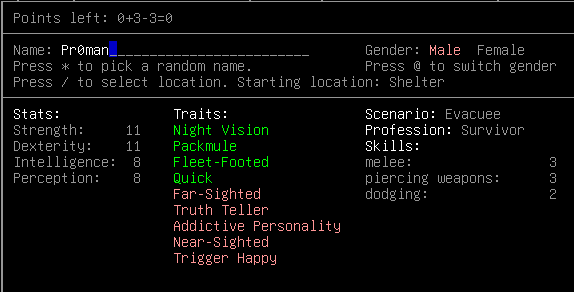
\includegraphics[width=\textwidth]{06}

For personal preference you are more than welcome to swap out anything you like, but I feel that from a combat-standpoint, this character can hold his own well, while also taking a weapon choice that is pretty good to start out with - though may be a bit annoying to craft unless you specifically head for it first.


\section{The Early Game}

So, we spawn into the world with our character, prepared to get our ass handed to us. First of all, let's check the map by pressing [m] - we need to assess the situation and see what should be the priorities:

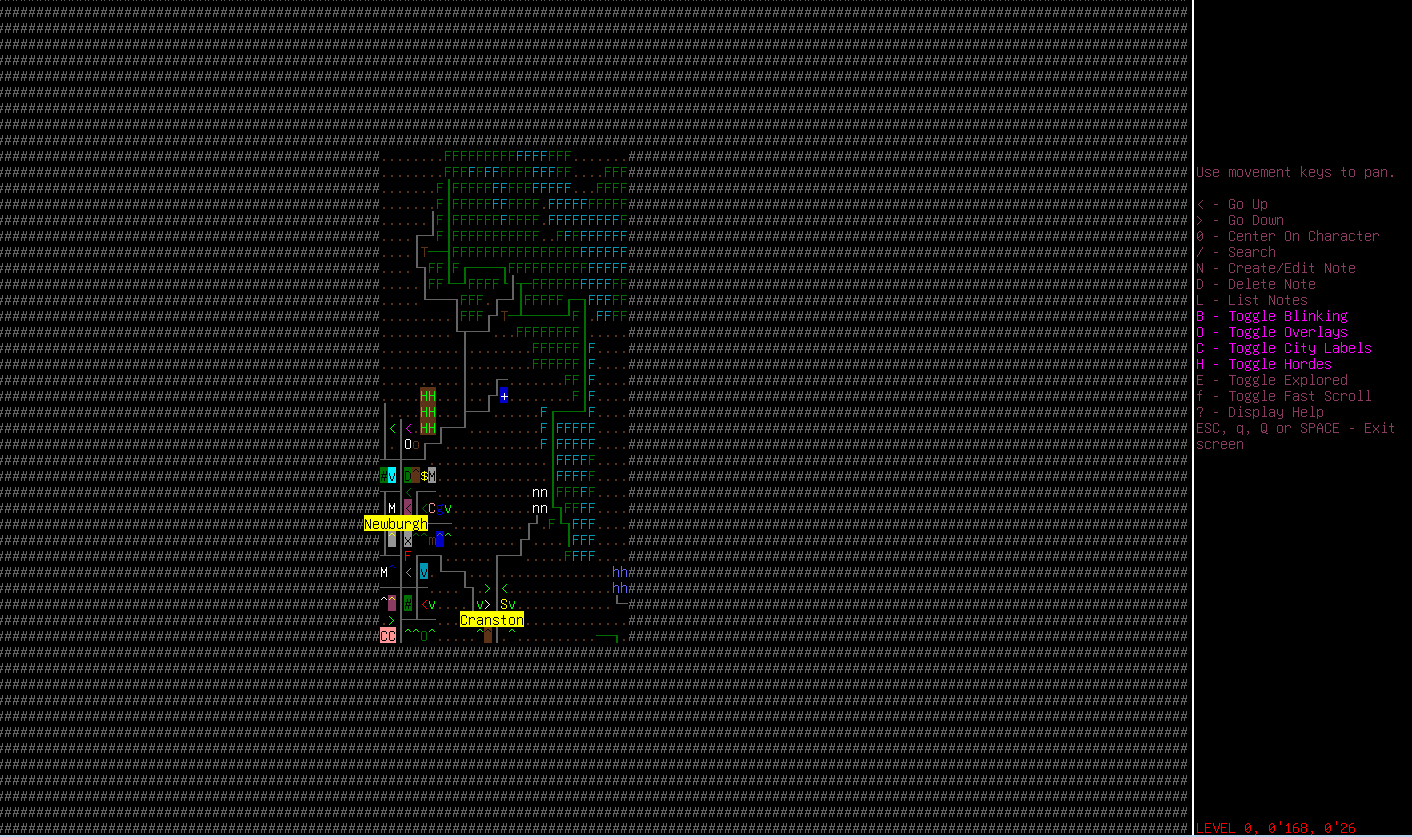
\includegraphics[width=\textwidth]{07}

As we can see, we spawned close to forests and swamps, which are intertwined with forest trails and relatively close to two cities, with some interesting structures in them - namely two libraries are visible.

However, this does not have to bother us yet. The most important things for survival are:
Water,
food,
gear,
in this order. So let us explore the shelter thoroughly.
A quick glance at the Terminal can however provide a bit of insight, we should definitely check it out and select the 'Contact Us' option so that we get a marker as to where the closest Refugee Center is, as well as a road marked towards it, if it is reachable by road.
The lockers can contain gear and utility items, mostly gas masks, first aid kits, emergency jackets and folded emergency blankets, while the basement usually contains a couple cans of food or random clothing, rarely some tools.

I got lucky in that I found a Jacket, Gas Mask and a Blanket - this will definitely keep me warm during the night.
The basement however, contained nothing at all, so, to secure water there are several options one can take - either sneak (or barge) into town, looking for cooking utensils like a pot or frying pan, as well as some containers to boil and store water gotten from the forest. Or, you could forage your survival up, hopefully find a can/bottle that has boiling quality and do pretty much the same. Since I play with wander spawns enabled, this is probably the safest option, as towns tend to spawn in lots of zombies and while my gear keeps me warm for the most part, it doesn't cover me in its' entirety and I will end up getting slowed sooner or later.

And just a couple steps to the north, right outside my shelter I already spot something:

\begin{center}
    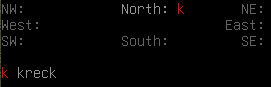
\includegraphics[width=0.5\textwidth]{08}
\end{center}

A kreck, not too difficult, but could at least damage my gear, however - and this is the important bit, where there are extra dimensional beings, there's loot to be had.

However, seems like there's more than just a Kreck, instead, a Mi-Go is right behind it. This is most definitely a fight I am not willing to risk. Those things hit hard, quite fast and you most likely will be unable to outrun them - that loot will have to wait.
So for now, let's head east instead, towards the swamp and see what we find - OH FUCK ME. A second Mi-Go.

\begin{center}
    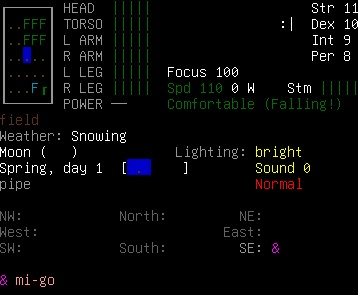
\includegraphics[width=0.5\textwidth]{09}
\end{center}

And while that may mean more loot, it means more places I need to tread extremely carefully, otherwise this run will end extremely quickly.

Well, I managed to sneak past it NE into the forest, after foraging to nearly rank 2 in survival and having no luck besides finding some veggies every now and then, I accidentally get too close to the first encounter location and aggro the Mi-Go. After a short run through the forests, I decide to try lighting a Bush on fire and to stand tall, or die here.

Lucky me, I survived' barely, my gear is messed, my head just as much, but I managed to deter the Mi-Go so it runs away in terror. It could've gone either way with the way Mi-Go's hit. So I just got lucky, this would've been a run-ender already. On the other hand, I can now loot the location.

Well, I found another plastic bottle of clean water - that will at the very least keep me going for yet another day, some Science IDs, which will definitely come in handy later, all that clothing on these 'overmap encounters' is also considered clean and comes with a decent amount of pockets. While I would always advise against going over encumbered, there isn't much I can do at this point but to grab all the things I can and hope for the best.
So in order for my vegetables and eggs to not rot away, I store them in the cellar and drop of the gear I collected somewhere (Certain foods go mushy if frozen and thawed, then rot away if frozen and thawed again)

On the other hand, I did manage to find some Rhubarb while foraging, this is totally fine to eat raw and comes with a nice bonus to our health stat (+3 each bite). That Trailhead [brown T] on the overmap might be worthwhile checking, as I spotted a car there'

Yup, there's a car there, a nice Pickup truck - lacks wheels though (and has a faulty engine, but nothing too bad), and on the radar I spot something next to it that looks like an RV.

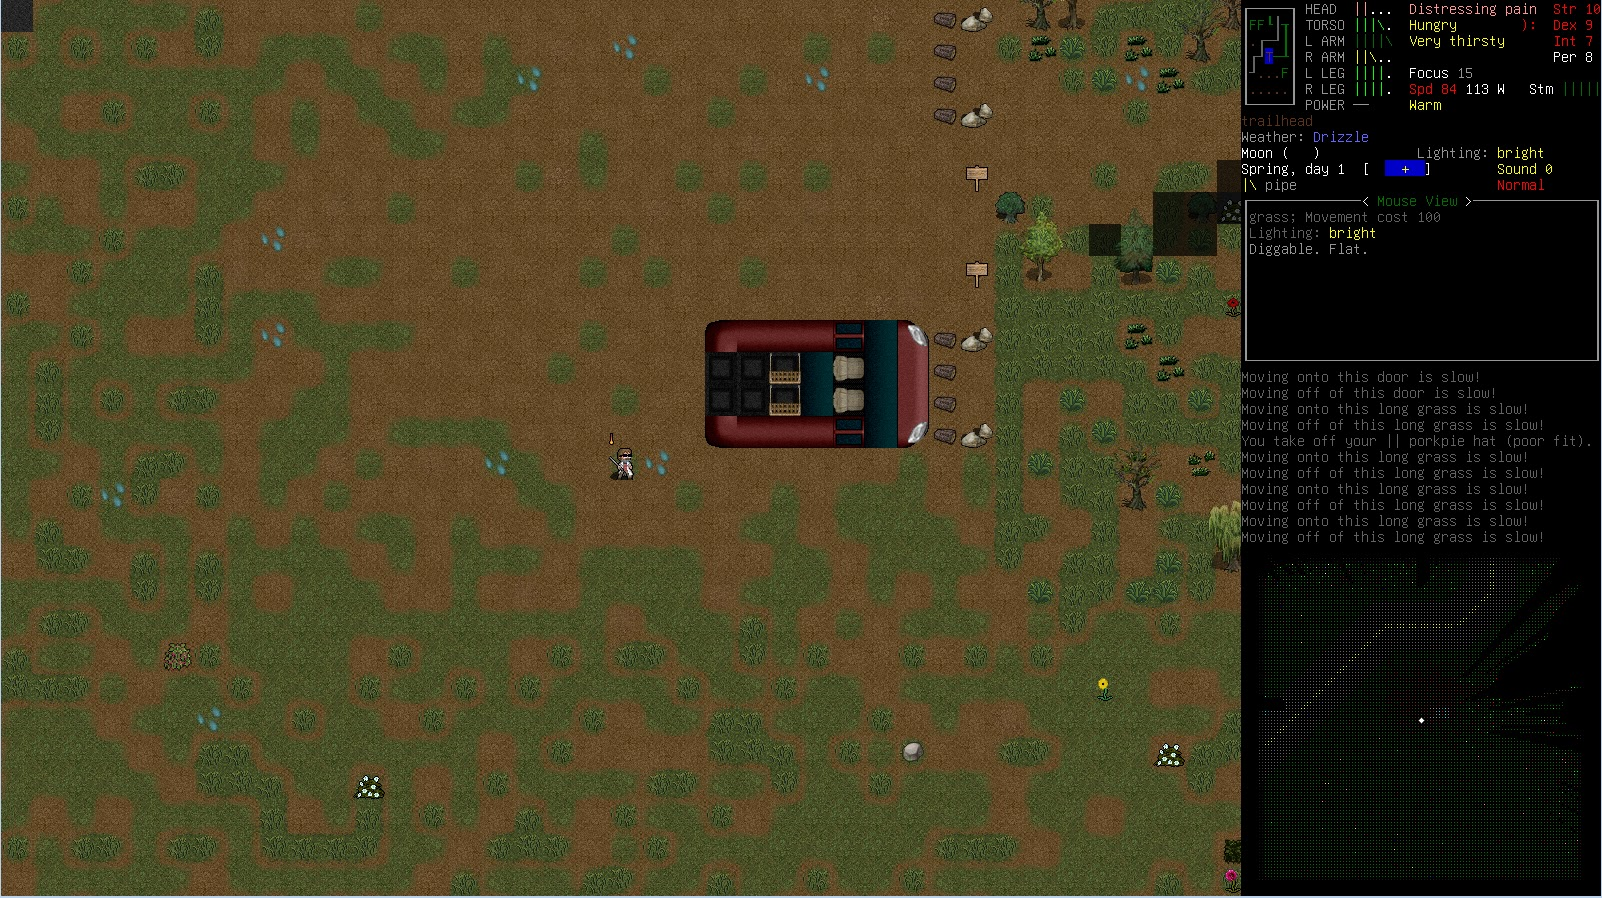
\includegraphics[width=\textwidth]{10}

Actually a meth lab, with a functioning chemistry lab. But it has no battery whatsoever inside, so no easy cooking for me. Guess it's up to more foraging and hoping for the best, as this is the only thing I can do now that I'm this beat up.

After foraging tile over tile in hopes of actually finding something with boiling quality, I decided to check out the forest trails for a bit, and look there, a glass bottle, I'm saved. Water is therefore ticked off of the list - why? Because A glass bottle is not just a container, but also able to be used to boil water in and with the 2 plastic bottles I found earlier, I also have a place to store it.

Well, it's getting dark - I basically wasted the first day looking for a suitable container to boil water with, which is nice, but it took so long and cost me lots of my HP that I'm gonna be hindered badly going forward, maybe. So, by cutting up some sheets that i tore down from the windows ([e]xamine), I craft myself some bandages till I hit tailoring of 1. Might as well go for it and apply them on each body part to gain some extra HP overnight. Before heading to bed, I'm gonna snack on the rhubarb I found earlier and have a drink to have a potentially easier time sleeping. And so I do and all of a sudden, I'm healed back to full, despite being torn up when heading to bed.

The next thing to work towards will be food supplies - while I did find lots of vegetables, eating those raw would be pretty bad for my mood, yet I can't cook them easily since they require Food cooking quality 2 to be turned into cooked wild vegetables. So, I need a better cooking utensil. Time to grab my bottles and head to a water source tile inside the forests'

By boiling water I can increase my cooking to 1, which in turn with my survival of 2 allows me to craft a stone pot, which is just barely enough and hey - I even managed to make that on my first try, even better. Time to cook some veggies. While I would prefer to have an indoor cooking place, a fire outside my shelter will have to do, as the floor is flammable and I don't want to torch down my only shelter.
(Sadly, the food rebalance update gimped this strategy of using wild veggies to keep your belly full. Making scrambled/boiled eggs works fine thou.)
Now with both water and food achieved, time to work on my gear, which means, I will have to work on my skills. After [s]macking up some benches I have enough nails and splintered woods to craft not only fishing hooks till I hit fabrications 1, but improvised fishing hooks till I am at fabrications 2, great start. A wooden needle for some sewing and our first proper weapon - a wooden spear. For that we need some long stick, so just smash a young tree till you get one after it is destroyed. The long strings from the curtains provide the thread from disassembling them into small strings and thread afterwards, rags come from the same curtains and a fire, like with cooking, we will gain by lighting up a splintered wood outside of our shelter (make sure there is 2 spaces in between you and the wall, you wouldn't want the fire to accidentally spread)

Time to work on some clothing, as what we currently wear is' well, less than optimal:

\begin{center}
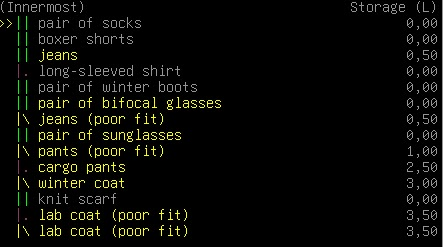
\includegraphics[width=0.5\textwidth]{11}
\end{center}

Yeah, that requires some work. good thing we made that needle and the bandages, with tailoring 1, we should have a somewhat easier time getting some gear up and running. So we grind our tailoring to 2 using pairs of light gloves (or any other recipe, it's all up to you) and at rank 2 we should definitely  make a long underwear top since that is close to the skin and therefore a great piece of clothing to wear as well as a balaclava to increase head and mouth temperature.
To grind further, I'd suggest using the T-shirt recipe, since that can also be disassembled instead of cut up, returning the full crafting resources.
Pr0-Tip: if you fail a couple of crafts, don't sweat it, the shelter has generally enough sheets to keep you outfitted for the first crafts that you do.
But why tailoring 3? Is clothing that important? Well, it is important in a sense that you require some pockets to store all the phat loots in, while also being free enough to be a force in combat, yet also not freezing to death. A clothing combo I'd suggest is a long underwear top, Duster and Backpack, Balaclava + boonie hat, some form of pants and respective boots. (the winter boots you spawn in quickly will turn your feet warm)

While sleeping, a zombie Cop decided it's time for an unannounced house search. So I promptly greeted him with my new wooden spear and he was so kind to leave me an AR-15 behind, oh goodie. While it's a bit dented, it will definitely come in handy.
Pr0-Tip: Remember that most spear-type weapons can be [f]ired in order to perform a ranged attack over 1 tile. The extra reach is what makes it for spears, while the armor piercing is more than welcome against semi-armored targets.

And on the start of day 3, this is how the clothing situation is now looking:

\begin{center}
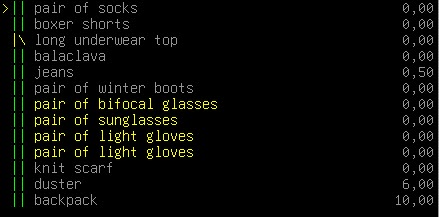
\includegraphics[width=0.5\textwidth]{12}
\end{center}

Well, I'm pretty happy with how things turned out. And since we are now properly equipped it's time to go exploring (we traded in a bit of defense from the winter coat for way more pockets and less encumberment all around) The spear makes for a great weapon against basically anything, except the zombie Soldier, but this is simply due to its' low damage values.

Pr0-tip - whenever you manage to kill zombie enemies, remember to pulp their corpses by [s]mashing the tile the corpse lies in. This will quickly stop them from reviving by themselves. This doesn't help against necromancers, but it works for now. And if this zombie is an acidic or spitter, don't pulp them, but perform a quick butchery once the acid is gone.

But, since there are some enemies I'd wish to soften up on range and I don't feel like wasting my precious .223 remington shots from my rifle, I'm gonna quickly craft a sling out of the 3 long strings all those curtains provide. (fabrication 1) Ammo is plentiful, just craft yourself a bunch of pebbles and you are all set to use it.
Even though the sling is considered a throwing weapon, it is used like any other ranged firearm, press [f] to fire, and aim according to your own tastes.
Quickfire tutorial on ranged combat:
[f] to enter firing mode
[.] to wait a turn and therefore stabilize your aim a bit.
[f] again to fire once you feel comfortable enough and waited the for you appropriate amount of turns.
or
while in firing mode:
[a] to aim and fire (medium aim)
[c] to carefully aim and fire (pretty good aim)
[p] to precisely aim and fire (best possible aim)
What these buttons do is wait a respective amount of turns until the aiming threshold is met, at which point, you issue a fire command.
Precise aim is what I personally go for - it takes the longest time, but maxes out your aiming and waits till recoil is reduced to 0, but therefore costs the most amount of time. Why? simple, not only am I pretty accurate in gauging the distance to enemies and how far they can move while aiming with different weapons - every shot missed means I wasted turns that the enemy could use to close the gap. And later down the line, when ammo is becoming a bit more common but still just a few touches too annoying to get, I want to make every shot count.
Nevertheless - why would I go for something so abhorrently weak like the sling? Well, turns out the Romans didn't use all these slings en masse for nothing. It is actually quite powerful and takes down normal zombies in just a couple hits. With ammo being basically infinite this makes for a nice first ranged option that also levels marksmanship for later.

So now most of the normal zombies become target dummies for my sling and wooden spear and I can technically start looting and clearing out towns. however, that superstore looks awfully tempting, but usually comes at the risk of being overrun by baddies. Doesn't mean I can't go take a look.

While checking the outskirts, I notice that the amount of zombies is way too many to potentially deal with. To the forest north is a helicopter crash site, right at the edge of the forest, Besides the zombie military pilot and soldiers, which already make this place unlootable for me, there's also a zombie bio-operator, something I will HAVE to avoid, as this could be run-ending.
So I venture further west, hoping of finding a nice entry way into the town, but mostly it's brutes, shockers or acidic zombies on the outskirts, far enough to potentially squeak through, but close enough that i don't want to take the risk. While walking back it appears as though the group of soldiers dispersed from the wreckage - turns out they guarded a poor fitting army helmet and an EMP. Well, whatever works. The dog they decided to maul gets field dressed first (to receive stomachs and offal) then fully butchered and that provides me with meat to my diet, while needing to be cooked first, the stuff will come in handy, especially the bones. The stomach that I managed to butcher will be turned into a sealed stomach, more water containers is a helpful benefit this early. While walking back, I noticed that to the SW of my shelter, there's also a Kreck running around, even more extra dimensional beings. I must've pissed off some sort of god to be this boxed in.

And while collecting water from my tile N-NE, I got attacked by the Mi-Go that I scared away on day 1 (btw, I was using a pipe from a smashed locker), looks like he wanted to go for another round, but this time, it was a fight to the death, for him. Though he did do a number on me and wrecked my clothing, torso and left leg and if that ain't enough, a spitter decided to show up just as I was about to craft the stomach. After quickly disposing of him, I sat down to lick my wounds, fix my gear and boarding up those windows, these zombies get awfully close.
Lucky that I found a hammer on one of the corpses and even if that wasn't a possibility, crafting a stone hammer at this point is no big task. As I started exploring the town SW of my location, i noticed a couple more wreckages and at this point I'm left wondering - is the world generation a tad borked? we'll see. Though as soon as I noticed obstructed vision on the radar, I knew there was something producing gas or smoke nearby, and yup, it's a smoker. Time to head back and actually grab the gas mask, prepare it and keep it on hand

Man, I seem to be getting extremely bad luck. While heading back, I nearly ran into a shocker brute and a normal brute by accident, luckily though I noticed them before they did notice me, allowing me to run as quickly as I could into the opposite direction - crisis averted.

After some approaches from different angles I managed to get towards a house on the eastern side, taking out a couple zombies on the way. Finally some building to ransack. Not only did the fridge have some edibles: A gallon Jug of milk and sandwiches of various kinds. But the oven I decided to bash out with my crowbar to obtain a sheet metal that will later be turned into a brazier, something that will contain fires, allowing for indoor cooking. Not only that, but amongst other things I found some drinks, more canned food, a desk fan and Atreyupan as well as other household drugs, which will be great if I ever happen to have a bite wound but no antiseptic medication on hand.

So it is now day 5
I'm pretty well situated for where I started out as, have some gear and food stocks, now I should work on scavenging together some tools and maybe look for a vehicle that would be worthwhile turning into a base.
Another factor in 'leaving' my shelter, speak my base behind, is the fact that the shocker brute is walking awfully close to it, and he has no trouble smashing up some house walls to get to my fleshy parts.

Well, what do you know, I did technically find a car that is drivable, a simple, plain car. Comes with a pretty battered fuel tank though, so it'll most likely leak gas everywhere. But in a pinch I could just ram the Shocker brute and be done with it.
But back to looting - while checking another house, an abandoned storefront and a gambling hall, I managed to come across a charcoal smoker (pretty useful for preservation), a real pot (finally some real cooking) as well as more food and a small book. Before I knew it, there were more zombies outside, guess they must've wandered in. One of them was nice enough to provide me with a toolbox, something I will gladly take at this stage of the game, as it combines most of the tools required into 1 handy item.
While this will come in handy - my assumptions happened: the car lost its' gasoline and now I have to haul things around. So I quickly turn some sheets from nearby houses into 2 makeshift slings, grab all my belongings and venture to the Military Surplus that is on the way. Not only do I find an Army helmet that actually does fit, but also the gun owners handbook as well as a plastic canteen, so now I can wear some water container on me at all times: The potentially best find could turn out to be the Leather Jacket as well as the hunting knife, as this knife is the best possible butchery tool easily available and the Jacket provides excellent protection, being made out of leather. Guess it's time to leg it back while assessing some cars and my potential options.

While considering what to do the next day, I decided to check out the Mobile Meth lab and to my dismay, it has no fuel tank, no battery and the engine has no drive belt. While that is in itself a minor inconvenience, the missing tank requires me to find or make a welder to replace that. But on the other hand, it would make for a great vehicle, not just coming with storage, but also a great vehicular station - the Chemistry Lab. So I decided to take a peek at the superstore, and to the road south of it, what do my sore eyes see? Another meth lab, only lacking some wheels - considering a Bottle Jack is way easier to come by, I'm most likely going to claim this vehicle instead, though it might be a bit parked in. Deciding to tackle to dollar store (which I mistook for a bank at first glance) I was able to grab me a shopping cart in perfect condition, meaning I now have a way of hauling around large amounts of items no problem, as well as finding a second canteen, so now all my water container problems are basically non-existent. Since the library was next door, I decided to head there, only to find several great books - The big book of first aid, Biodiesel: the renewable fuel source, A history of Firefighting, how to trap anything, the book of dances and last but not least The historic weaponsmith(!) this will most likely proof to be extremely valuable, as this'll allow me to craft medieval weapons of all kinds that have quite the punch to them - from a Morningstar and Mace to the Estoc, Halberds, Glaives, different kinds of swords, the Awl pike (though that one was nerfed terribly as of recently). This will come in real handy real quickly. The only problem is gonna be managing to get a forge and maintaining said forge. But I might as well start working on this. The fabrications skill is easily obtainable by grinding certain crafting recipes (Distaff and Spindle - Pair of wooden Clogs - Banded wooden Cart wheel), this way, I can easily reach fabrication 5 in two days' work, while my supplies keep me covered. Drinkables are a non-issue at this point, as is food - animals in somewhat close proximity to the shelter can quickly be killed (except for moose or bears), butchered and turned into food.

So not only did we tick off the most pressing needs in form of water, food and gear (god that toolbox drop) as well as shelter - the starting evacuee shelter makes for a great makeshift base of operations to start out with, but we also managed to scout out some vehicles, are about to set up a forge to allow for some extra weapons as sidearms to switch to and can freely grind any skill we like, as not many enemies at this stage pose much of a threat, with the exception to shocker brutes and enemies bigger than that.

Due to being settled in properly, I'd suggest that this is the end point of the early game and we can say we clearly moved towards the mid game.

\section{The Mid Game}

Day 8 - not a bad situation to be in, as I not only have a toolbox, several great books to boot, a vehicle scouted out and lots of permanent food in the form of cans as well as several animals running around close to the shelter if I ever want something more fresh.
However, as I was grinding skills, a horde apparently decided to walk around my shelter as there's been several shockers in that group, one of them a brute. So, nighttime combat it is then - the spear easily deals with most of the enemies, except those electrical ones. those I take out with a sling, many pebbles and lots of dedication. At dawn I check the aftermath of the murder to loot, pulp any zombies I missed and start heading out for the next day - couple pieces of loot include:
-ammo + a single barrel shotgun
-electrical tools (flashlights, tazers, radios)
-a mini freezer (sweet)
-several drugs, aspirin, cough syrup and so on.

Since I'm wanting to make a forge setup, as I do require better weapons at this point, I'll have to collect lots of rocks, 80 at least. I'm gonna go with the safer approach of checking the forests for small boulders to bash down (1-6 rocks each), as torching a building would cause many enemies to get spawned nearby (wander spawns) and maybe stopping short of the fire, leaving the area difficult to reach.
This also has the added benefit of gaining some extra food items to eat so that I can save my permanent food items for a bit longer.
Collecting all those rocks took me a day, but depending on luck might require more time - careful when doing this at night, a moose decided to watch me.. a bit closer than I'd have liked, so I decided to poke him with my spear and turn him into edibles
So, for a proper forge setup, we require:
-Charcoal kiln
-Rock forge
-several tools
The Kiln and forge are no problem, while we construct the forge, I also filled up the kiln with a bunch of sticks I collected from young trees outside the base.
However, now we need metal, lots of it. While having the toolbox makes this really easy to get (just remove vehicle parts like doors for frames), we can also check wreckages to see if there's already bashed out frames, as well as collecting lots of scrap. After bringing over a sufficient amount of metal in forms of frames (5), a sheet metal and lots of lumps/chunks, we can forge ourselves the tools required to operate a forge - crucible, anvil, metal tongs, metalworking chisel and a swage an die set -, an entire toolset, which we luckily won't need, and also more importantly - bigger weapons.

As for that part - I'd suggest any player to go with a Steel Spear, simply due to its superior range. Which is also what I'll be going for, as it makes dispatching shocker brutes totally possible.

Next up on the list is looting that nice home improvement Superstore next door while also cleaning that one out a bit.
And while it wasn't all too difficult all things considered, the loot was pretty worth it - lots of spare parts, mostly nails and copper wire, some utility tools like bolt cutters but by far the best loot in it was a telescopic crane mounted on a foldable frame, meaning I now have some lifting and jacking quality at hand which can be stored away nicely.

Since we did have that RV in pretty decent condition only lacking wheels, time to look around the different kinds of cars in order to find some wheels. While 32' wide wheels would be great right about now, anything will do, even some 17' normal wheels. However, to do any sort of work related to vehicles, I need skills - while I have a mechanics book for range 3 - 6, I need mechanics 3, and electronics won't hurt either, so time to just do some general looting.
Good thing there was still a library just a couple minutes walk south - in it were lots of great books, same with the surrounding housing - Mechanical Mastery, Sewing Techniques for Designers as well as the Clothing Designers Portfolio, Ham Radio Illustrated and What's a Transistor. I ought to play the game more often on easier settings, sure feels good.
Anyways, the two electronics books are quickly read, giving me access to a soldering iron, Under the hood provides me with mechanics 3, and there's the welder already, even with battery compartment mod due to one of the electronics books having it.

After stocking up on car batteries, trying to find some wheels (those must've been the first thing to get hit by the cataclysm, I had a really hard time tracking any useable wheel down) and even managing to find 3 solar panels, I decided to bring a batch of food and water with me, i'm gonna do some mechanics work.

Mostly uneventful except for the odd zombie showing interest in my finesse with the tools. Installing wheels and [c]hanging them where it's necessary sure took its time. Slapping on the solar panels that I found will at least, over time, recharge my car batteries that I'm inevitably drain using the welder. Took me two days straight to get the thing up and running, since, hell, might as well upgrade it a bit and the low-end cube van right next to it provided some sweet cargo spaces to increase my loading capacity. After I get this thing to run properly, I [s]iphon some gas from the nearby vehicles and drive back to my makeshift base, which is the evac shelter. Since I'll be planning to live on the road in order to explore many different features, we'll be abandoning this camp, so time to pack up - I made some makeshift slings and wore another backpack and went packing, sorting everything properly. Now that that's out of the way, let's get to reading up all those books. Skills matter, and if I wish to forge some weapons, an electric forge with a compartment mod is my best bet at this point. The remaining charcoal that I made will be used for the small charcoal smoker I found earlier. Good thing there was this home improvement superstore - the ovens in there will be handy to get the heating elements I need.
But like I said - skills are survival, without better combat skills I will be stuck against bigger enemies, without better armor, which I can now craft thanks to those books, I will constantly take damage and without late game power tools I will have trouble breaking and entering late game structures.

While reading, I totally did not notice that one of the books I looted appears to give me the weapon arts 'Fencing', so I guess instead of going for an Estoc, I'll make a broadsword instead as it is a compatible weapon for this style. Having multiple melee options is not a bad thing anyways. So off to more looting, resources for better armor are not just acquired overnight, at least for the most part.

While cleaning out the city I noticed some acidic soldier ants at the NW edge of town. Seems like I found myself a nice playground for the later stages of the game.

\section{The Late Game}


\chapter{Tips and Tricks, FAQ}

So, you either skipped to this spot or decided to read through the entire Guide and are now interested in some quick tips for certain things. Or maybe you wonder if a question you might be asking yourself will be answered here? We shall see. For those wondering why absolute base questions pop up here, even though they have been answered - this is for those absolute beginners that want to experience the game on their own, but are wondering why certain things don't work out for them as they expect.

\textbf{Q:} How to I raise (insert skill here) from (insert level here)?\\
\textbf{A:} Either by finding books (unlikely to find the exact book you are looking for) or by performing the appropriate action. Combat skills raise naturally and you have to chin it up for the most part, as books only get you so far, but for anything crafting related, the biggest tip I can give to you is this - use the recipe search [f] while inside the crafting window.

By searching using a parameter you can easily find what you should be crafting in order to specifically raise a skill - So if you require fabrications, do 's: fab' in order to find a recipe that has the skill fabrications required and search through the list. Works with any skillname, either partly or in full. Remember that there aren't recipes for each level that are automatically learned, this is meant to incentivise you looking for books or learning the skill out in the wild.

\textbf{Q:} How do I raise mechanics from 0?\\
\textbf{A:} The classic one, since mechanics from 0 is somewhat more difficult to raise, as you won't find recipes relating to it in an unmodded game, or with some side-skills taken at the very start.

My general suggestion - make 4 wooden frames, have 40 nails around and create 2 vehicles (construction menu), after starting the vehicle, install a wooden box into the 1 tile (make sure you have high focus for this, otherwise it'll take more)

This usually gets you to mechanics 1, at which point you can uninstall/install smaller parts from existing vehicles using a screwdriver.

\textbf{Q:} Why do my shots keep missing even at close range?\\
\textbf{A:} Make sure to aim by waiting [.] or use one of the appropriate aiming options in the firing menu. [a]im, [c]areful aim or [p]recise aim respectively.

\textbf{Q:} How do I cook food and heat up existing food?\\
\textbf{A:} use the crafting menu [\&] and select what you wish to create. To heat up food, you require a tool you need to activate (Frying Pan/Pot/Stone pot etc.) and either a fire or tool that can work for heating (Hotplate, Mess Kit etc.)

\textbf{Q:} Why am I sick?\\
\textbf{A:} General sicknesses like the common cold of flu just happen, unless you wear a gas mask or similar constantly, avoiding those is gonna be next to impossible. If you got poisoned or food poisoning, this happened because the food you decided to throw into your system wasn't meant for eating raw. Some enemies can also infect you with disease-like status effects.

\textbf{Q:} How do I run from zombies?\\
\textbf{A:} Press ['] to toggle between walking and sprinting. Also make sure to break line of sight, even though zombies can track you using scent, their vision is the most important sense.

\textbf{Q:} How do I loot towns?\\
\textbf{A:} be creative! Use fire to torch an already looted building to attract zombies to burn to death, raid at night (carries its' own risks), or just run through it with a pair of rollerblades while dragging a cart behind you.

\textbf{Q:} Why can't I hit stuff in melee?\\
\textbf{A:} Either you lack the skill in your weapon category or (more likely) you are too over encumbered with your gear. Encumbrance is king when it comes to combat and you will have a hard time hitting an enemy with 2 backpacks and 2 makeshift slings worn. So feel free to read the section 5.3.2 Temperature and Clothing to get a general idea of how clothing affects you, or 5.3.5 Combat to get a better grasp of combat.

\textbf{Q:} How do I train my skills?\\
\textbf{A:} Not only was this answered as the very first question, but again. Use them! Every action performed that is linked to a certain skill will increase it naturally, or if you happen to find a book, read that.

\textbf{Q:} Something keeps hurting me but I'm not being attacked or anything?\\
\textbf{A:} You most likely have caught a parasite by eating raw meat. Curing that requires some antiparasitic drugs.

\textbf{Q:} I'm infected, what do I do?\\
\textbf{A:} Pray to whatever higher being that you will survive. If you are however an atheist, your best, and only option at this point are to find some Antibiotics or Royal Jelly to cure the infection. Atreyupan is only a prophylactic measure and can't cure infections, only slow them down, prolonging your time window from 24hrs to 48hrs. Your best option is to not let deep bite wounds get to the point of being infected.

\textbf{Q:} How do I stop getting infected?\\
\textbf{A:} Any deep bite that you obtain will turn your limb from the normal white Name (i.e. TORSO: \textbar\textbar\textbar\textbar\\) to a blue coloured name. This can also be seen in character overview [@] under status effects (the bottom right part of the window). When you are at this stage, a deep bite wound can either be cleaned using any form of disinfectant (disinfectant, makeshift disinfectant, hydrogen peroxide) on said limb, or it can heal naturally over time. The chance for a bite healing on its own is based on your hidden health stat, so eating and living healthily has its benefits, still, your best option is to carry around a small bottle of disinfectant for on the spot cleaning of wounds.

\textbf{Q:} Where can I get a long-term water supply?\\
\textbf{A:} Forests contain water tiles you can fill containers in, if those aren't an option - swamps either have salt- or freshwater in them, but usually always contain both somewhere so make sure to check every water tile, even connected ones. If nothing like that works, you can just use a funnel on an open tile and place a water container below (drop it on the same tile).

\textbf{Q:} How do I control a vehicle?e\\
\textbf{A:} [\^] on the driver's seat. If you wish to learn more about vehicles in general, check section 5.3.11 - Vehicles.

\textbf{Q:} Why do I keep dying in combat?\\
\textbf{A:} First of all - Welcome to Cataclysm, hope you'll enjoy your stay. But to answer the question - combat has several factors that can easily decide a battle on their own (Pain, Encumbrance, difficulty of Enemy etc.), please feel free to read about combat in the appropriate section.

\textbf{Q:} I just started out but idk what to do.\\
\textbf{A:} This ain't a question but rejoice nonetheless! Read through this tutorial in its entirety please.

\paragraph{More unassorted tips:}
\begin{itemize}
\item Make a sling early game for ranged combat and fire pebbles at enemies, it is surprisingly strong against unarmored targets. Anything that is armored will give you trouble thou.
\item If you can't find a shopping cart, make your own by using 2 wooden frames (just a vehicle frame + wooden box on the same tile), will create noise when dragged, but it is storage.
\item Beware that most buildings that would have an alarm system in real life come with an alarm system in the game, not only attracting zombies nearby, but calling in eyebots. (houses excluded)
\item Whats unhealthy in real life is most likely also unhealthy in game.
\item Pick your fights carefully, Just because you can beat 3 zombies in a group, doesn't mean it is the same with 3 Zombies + 1 Spitter Zombie
\item You need lifting quality for a vehicle part? Just weld a forklift arm (requires steel frame) on to any frame and drag that along. How you can weld a metal piece onto a frame made out of wood, I have no clue.
\item Always keep some medical supplies handy - having to run back to your base because you forgot antiseptic is bad enough as is, but bleeding to death because you didn't want to carry 3 bandages with you is your own fault.
\item Peek around building corners using [X] - enemies will most likely not notice you doing so.
\item The game runs only when you decide to. Take your time and assess your situation to check every possibility.
\item While prioritizing what loot is important is a good thing, make sure to get a general idea of what is used as a component for crafts and where to obtain it.
\item On that note, read the item descriptions and its additional modifiers carefully! Countless newer players used fake medieval weapons only to wonder why they sucked so much using it.
\item Deconstruct furniture (construction menu) instead of [s]mashing it for getting the most resources out of it.
\item Electronic components can be obtained from Terminals, Arcade Machines, Washing Machines/Dryers. Ovens carry Heating Elements.
\item If you have trouble keeping your food fresh for long, try building a Root Cellar or finding a frozen Science Lab, which will cool your food below freezing point.
\item Need a Distraction? Anything creating noise is great, like a two-way radio, firecrackers or a noisemaker to draw zombies from one location to another - works especially great at night so just activate and throw
\item Vehicles are the solution to most of your problems - Locked doors? Ram it. Zombie Hulk? Ram it. Low on food? Insert vehicle at high speed into edible animal.
\item Turrets and various kinds of robots are actually your friends. Not only are they pretty well armored, they also come with several firearms equipped to deal with the nasty hordes of the apocalypse. Just drag zombies into the more tame ones (like eyebots) while trying to get away, make sure to break line of sight and to NOT walk into those robots. The last thing you want is you riddled with bullet holes from a tank drone.
\item Same works for animals - if you can manage to position yourself between a moose and some zombies, by running ['] quickly past a Moose or Bear in a circle motion, you can make the zombies take a path that is a smaller circle and way more likely to get too close to said animal. Just make sure YOU don't get too close to it.
\item Get to the habit of remembering your vehicles position [K] when [e]xamining it. The last thing you want to do is to search for your shopping cart that you have left behind because you were chased or you simply forgot.
\item Vehicular tool stations are off-limits to you? No Problem. A couple solar panels on your car, coupled with extra car batteries got you covered. Just install a Battery Compartment Mod into the most commonly used tools (Welder, Forge, Food Dehydrator, Food Processor) and load them up with car batteries.
\item Maximize butchering outputs! A Metal Butchering Rack is not difficult to make at the mid game and allows you to create a butchering station on the fly. Keep a couple 2x4's and nails on hand to construct a table, or make the Tourist Table for a deployable one. This also means having high butchering quality helps drastically - a Hunting Knife is the most powerful tool that does not require batteries.
\item It's headed right towards you? Yell at it [C]! Many animals are scared by loud noises and can therefore be deterred by yelling at them. This only works for natural wildlife, so deer(which are already afraid of humans) and bears - and even then it doesn't always work, but hey, it might just save your life. Wolves can not be feared by noise, and as of recently, the noise trigger for moose has been removed.
\end{itemize}

To recap: do NOT be afraid to play carefully: [X] to peek around corners, [e]xamine closed windows that have their curtains pulled in order to peek out of them and run whenever you feel like you don't want to take a fight - there's no shame in surviving.

\end{document}
